\documentclass[9pt]{beamer}


\mode<presentation>
{
\usetheme{Singapore} %use default if problems or  Singapore or 
  % or ... https://deic-web.uab.cat/~iblanes/beamer_gallery/index_by_theme.html
\usefonttheme{serif}  
}
\setbeamertemplate{footline}[frame number]
\usepackage{booktabs}
\usepackage{color}

\usepackage[english]{babel}
% or whatever

\usepackage[latin1]{inputenc}
% or whatever

\usepackage{times}
\usepackage[T1]{fontenc}
% Or whatever. Note that the encoding and the font should match. If T1
% does not look nice, try deleting the line with the fontenc.
\usepackage[super]{nth}
\usepackage{xcolor}
\usepackage{relsize} %large math 

\usepackage{graphicx} % to insert the logo

\usepackage{hyperref}
\hypersetup{
  colorlinks   = true, %Colours links instead of ugly boxes
  urlcolor     = blue, %Colour for external hyperlinks
  linkcolor    = blue, %Colour of internal links
  citecolor   = red %Colour of citations
}

\usepackage[font=scriptsize,skip=1pt]{caption}

\setbeamertemplate{caption}[numbered]

\title[Nuovi modelli] % (optional, use only with long paper titles)
{Nuovi modelli, dalla diffusione della Covid-19 all'agricoltura di precisione}

\author[] % (optional, use only with lots of authors)
{P.~\href{https://terna.to.it}{Terna}\inst{1~2~3}  }
% - Give the names in the same order as the appear in the paper.
% - Use the \inst{?} command only if the authors have different
%   affiliation.


\institute[] % (optional, but mostly needed)
{
  \inst{1}%
 University of Torino, Italy
  \and
 \inst{2}%
  Fondazione Collegio Carlo Alberto, Honorary Fellow, Italy
  \and
  \inst{3}%
  Accademia di Agricoltura, Torino, Italy
 }
% - Use the \inst command only if there are several affiliations.
% - Keep it simple, no one is interested in your street address.

\date[] % (optional, should be abbreviation of conference name)
{\href{http://www.accademiadiagricoltura.it}{Accademia di Agricoltura}---10 novembre  2021, slides at \url{https://terna.to.it/aa.pdf}}

\begin{document}

%%%%%%%%%%%%%%%%%%%%%%%%%%%%%%%%%%%%%%%%%%%%%%%%%%%%%%%%%
\begin{frame}


\includegraphics[width=0.08\textwidth]{logo2_unito.png}~~~~~~
\includegraphics[width=0.08\textwidth]{CCA_Logo2.png}~~~~~~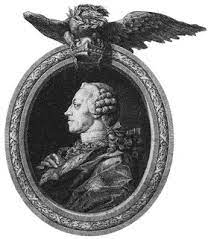
\includegraphics[width=0.07\textwidth]{A_agr.jpeg}


\titlepage


\end{frame}

%%%%%%%%%%%%%%%%%%%%%%%%%%%%%%%%%%%%%%%%%%%%%%%%%%%%%%%%%
\begin{frame}{Outline}

  \tableofcontents
  % You might wish to add the option [pausesections]
\end{frame}

%%%%%%%%%%%%%%%%%%%%%%%%%%%%%%%%%%%%%%%%%%%%%%%%%%%%%%%%%
\section{New models}

%%%%%%%%%%%%%%%%%%%%%%%%%%%%%%%%%%%%%%%%%%%%%%%%%%%%%%%%%
\subsection{Agent--Based Models}

\begin{frame}{Introduction}

\begin{figure}[H]
\center
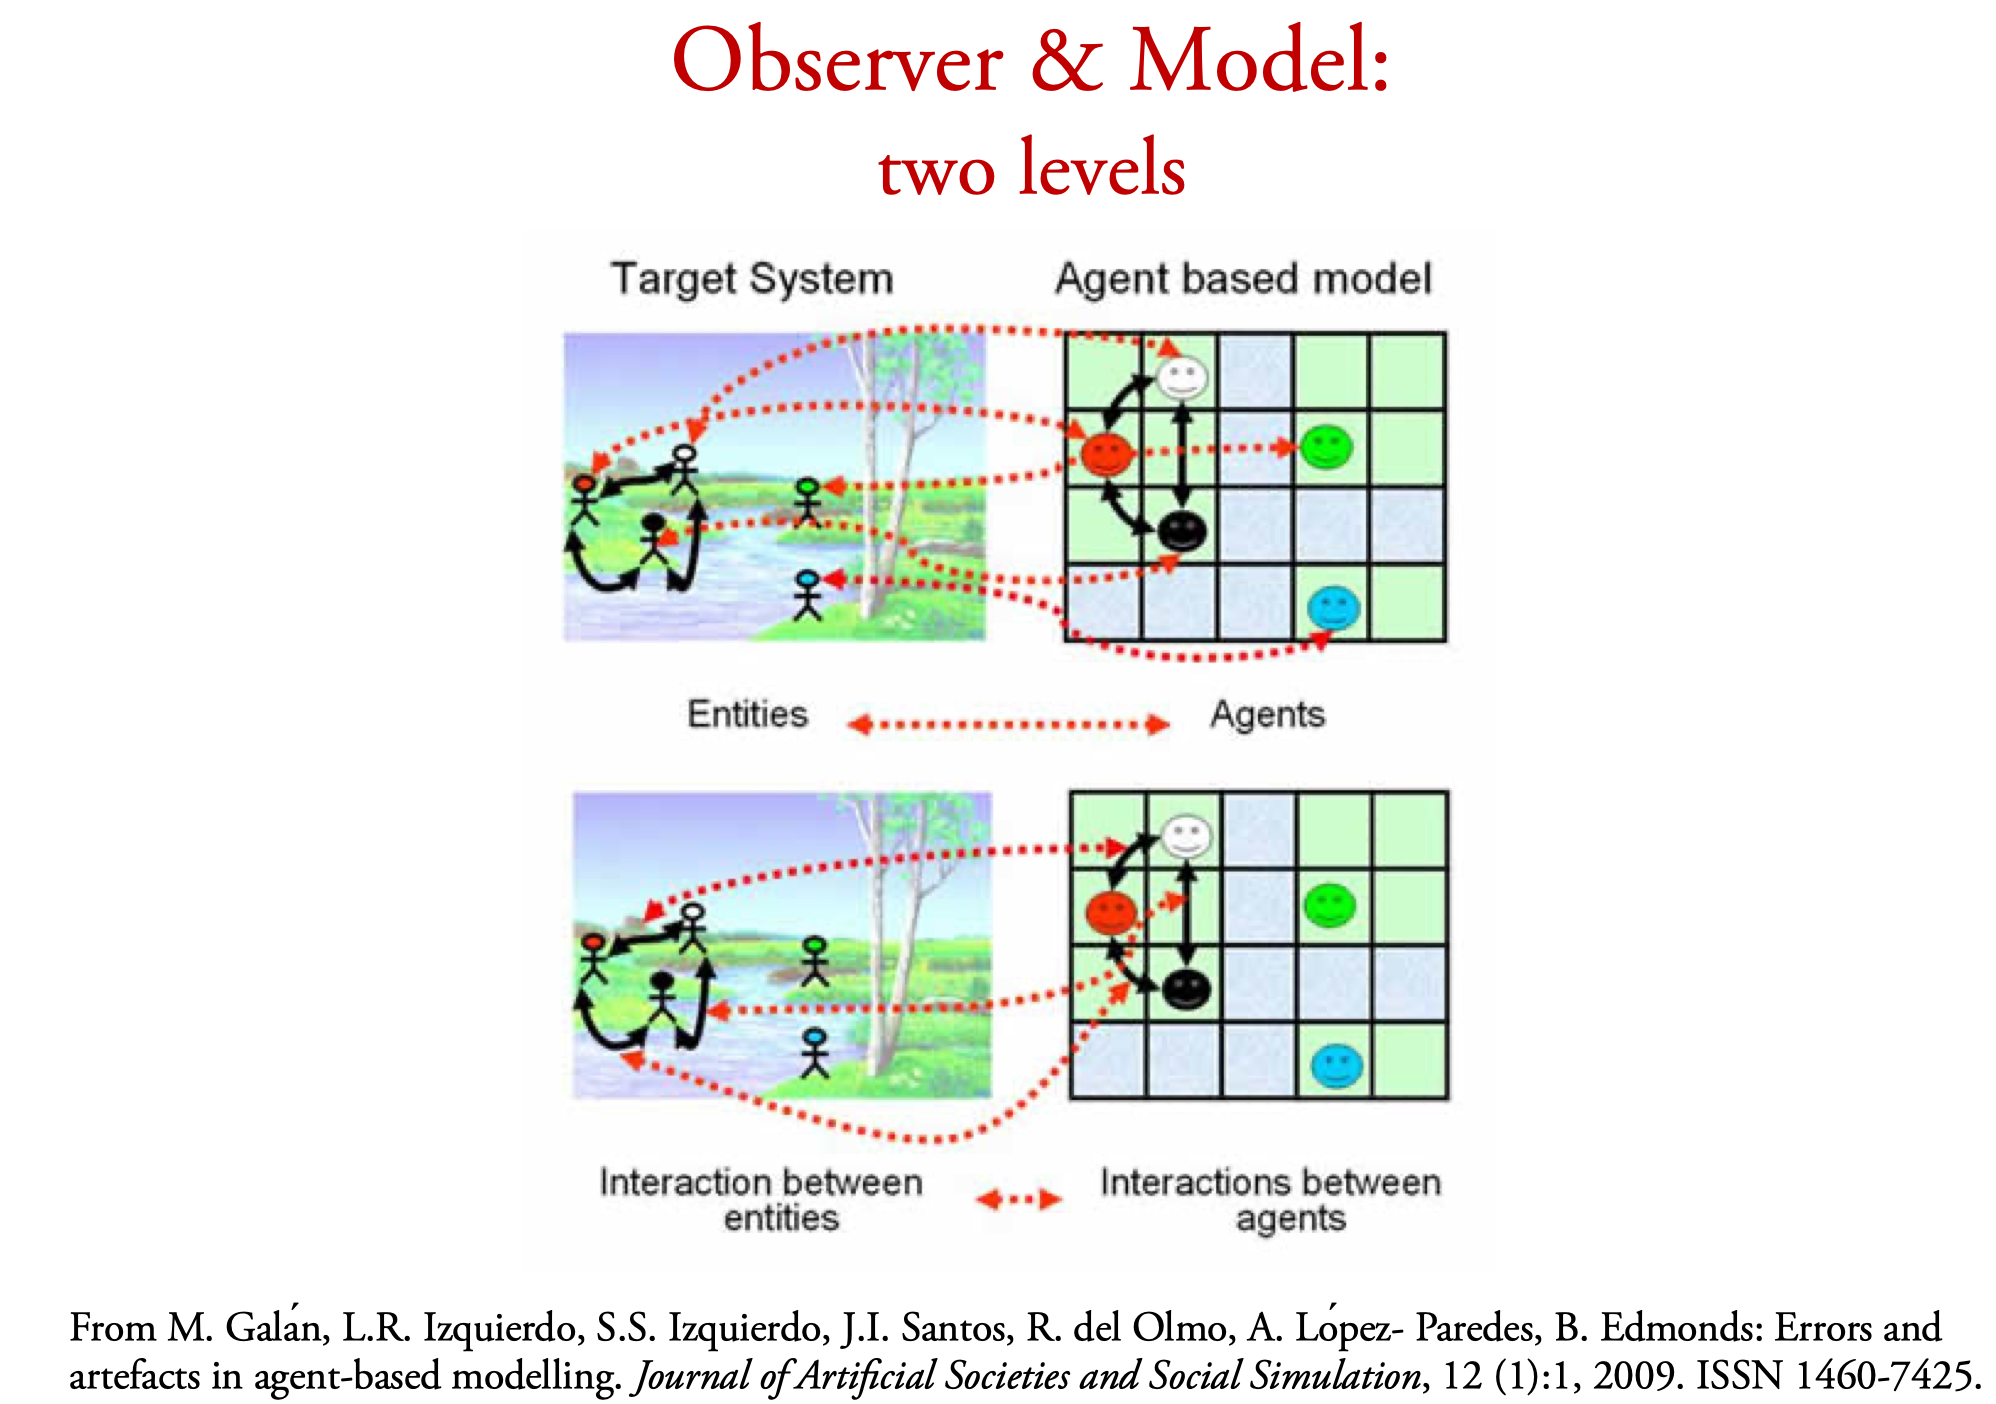
\includegraphics[scale=0.27]{abm1.png}
\label{abmPicture}
\end{figure}
\url{http://jasss.soc.surrey.ac.uk/12/1/1.html}

\end{frame}


%%%%%%%%%%%%%%%%%%%%%%%%%%%%%%%%%%%%%%%%%%%%%%%%%%%%%%%%%
\begin{frame}{Tools}

\begin{figure}[H]
\center
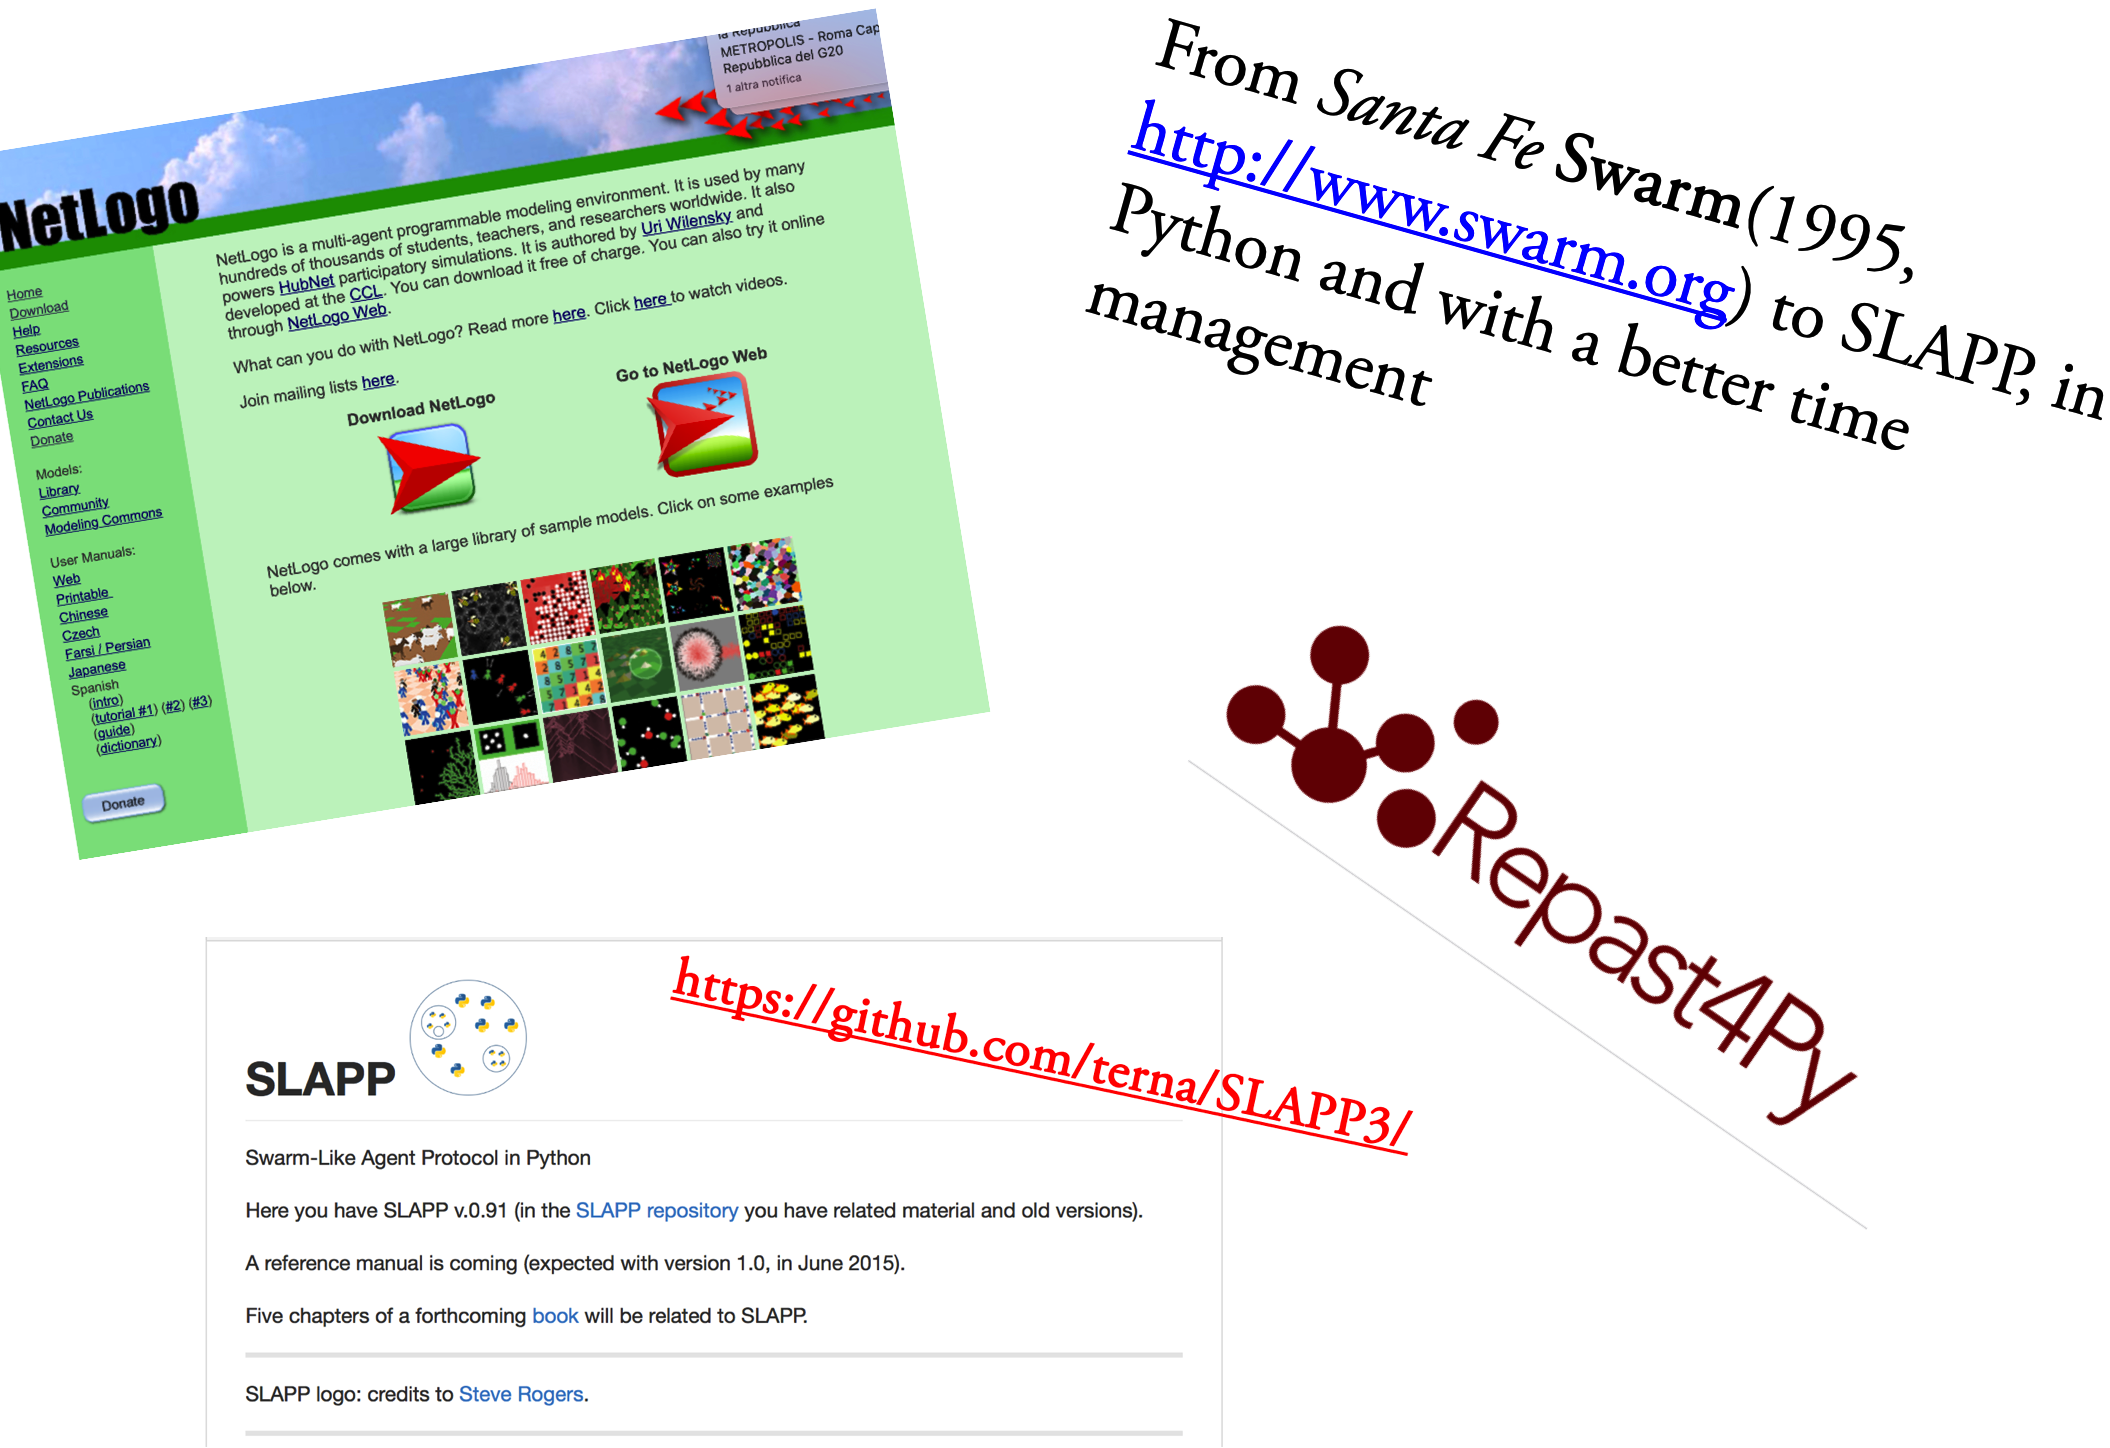
\includegraphics[scale=0.14]{tools.png}
\label{tools}
\end{figure}


\end{frame}

%%%%%%%%%%%%%%%%%%%%%%%%%%%%%%%%%%%%%%%%%%%%%%%%%%%%%%%%%
\begin{frame}{Scheme}

\begin{figure}[H]
\center
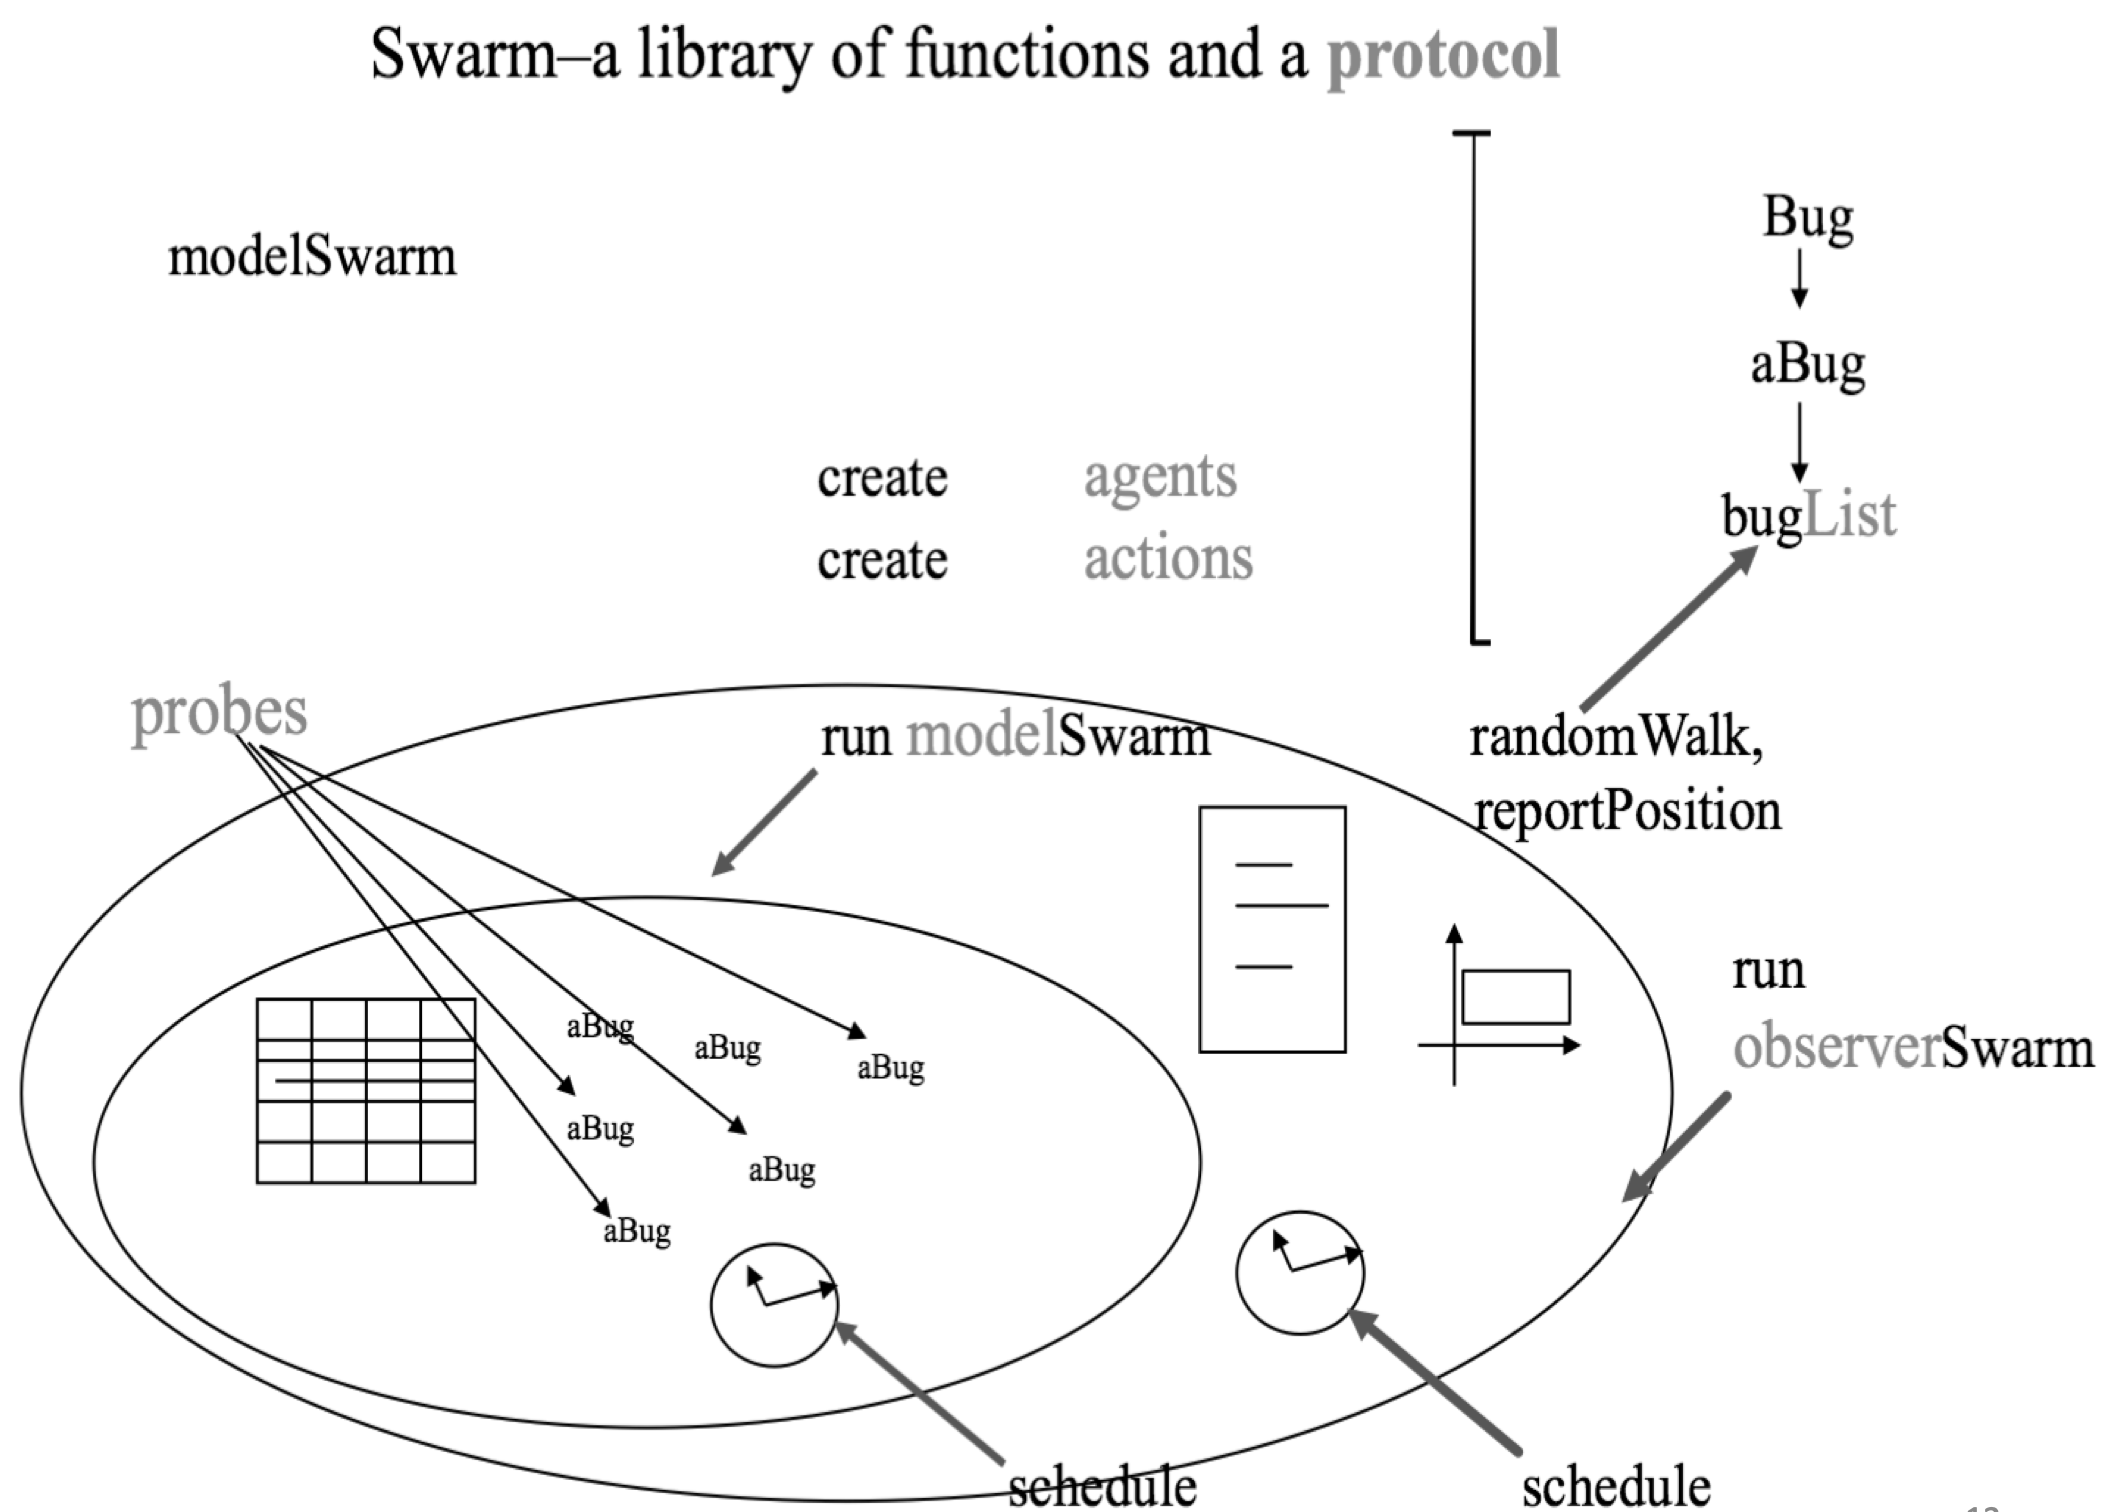
\includegraphics[scale=0.26]{scheme.png}
\label{scheme}
\end{figure}


\end{frame}

%%%%%%%%%%%%%%%%%%%%%%%%%%%%%%%%%%%%%%%%%%%%%%%%%%%%%%%%%
\section{The virus model}

\subsection{An ABM on virus diffusion}

%%%%%%%%%%%%%%%%%%%%%%%%%%%%%%%%%%%%%%%%%%%%%%%%%%%%%%%%%
\begin{frame}{An ABM on virus diffusion: a paper describing the model}

G. Pescarmona, P. Terna, A. Acquadro, P. Pescarmona, G. Russo, E. Sulis, and S. Terna. \emph{An Agent- Based Model of COVID-19 Diffusion to Plan and Evaluate Intervention Policies}, 2021. \url{https://arxiv.org/abs/2108.08885}.


\end{frame}


%%%%%%%%%%%%%%%%%%%%%%%%%%%%%%%%%%%%%%%%%%%%%%%%%%%%%%%%%
\begin{frame}{Introduction}

\begin{itemize}

\item
A micro-based model of interacting agents, following plausible behavioral rules into a world where the Covid-19 epidemic is affecting the actions of everyone. 
\item
The model works with: 

\begin{enumerate}[i]
\item infected agents categorized as symptomatic or asymptomatic and 
\item the places of contagion specified in a detailed way, thanks to agent-based modeling capabilities. 
\end{enumerate}

 \item
The \textcolor{red}{infection transmission} is related to three factors: the infected person's characteristics and those of the susceptible one, plus those of the space in which a contact occurs.

\end{itemize}
\end{frame}

%%%%%%%%%%%%%%%%%%%%%%%%%%%%%%%%%%%%%%%%%%%%%%%%%%%%%%%%%
\begin{frame}{~}

\begin{itemize}
\item
The micro-based structure of the model allows factual, counterfactual, and conditional simulations to investigate both the spontaneous or controlled development of the epidemic. Examples of counterfactual situations are those considering:

\begin{enumerate}[i]
\item different timing in the adoption of the non-pharmaceutical containment measures;
\item  alternative strategies focusing exclusively on the defense of fragile people.
\end{enumerate}

\item
The model generates complex epidemic dynamics, emerging from the consequences of agents' actions and interactions, with high variability in outcomes, but frequently with a stunning realistic reproduction of the  contagion waves that occurred in the reference region. 

\item
We take charge of the variability of the epidemic paths within the simulation, running batches of executions with 10,000 occurrences for each experiment.

\end{itemize}
\end{frame}

%%%%%%%%%%%%%%%%%%%%%%%%%%%%%%%%%%%%%%%%%%%%%%%%%%%%%%%%%
\begin{frame}{~}

\begin{itemize}

\item The \textcolor{red}{AI and inverse generative sides of the model} come from constructing a meta-agent optimizing the vaccine distribution among people groups---characterized by age, fragility, work conditions---to minimize the number of symptomatic people (deceased persons come from there).

\item We can characterize the action of the planner both:
\begin{enumerate}[i]
\item introducing ex-ante rules following ``plain'' or ``wise'' strategies that we imagine as observers or
\item \textcolor{red}{evolving those strategies via the application of a genetic algorithm}. 
\end{enumerate}

\item The genome is a matrix of vaccination quotas by people groups, with their time range of adoption. 

\end{itemize}


\end{frame}

%%%%%%%%%%%%%%%%%%%%%%%%%%%%%%%%%%%%%%%%%%%%%%%%%%%%%%%%%
\begin{frame}{The model}

\begin{itemize}
 
 \item
As the agents can be Susceptible, Infected, symptomatic, asymptomatic, and Recovered, the name of the model is S.I.s.a.R., with the capital letters recalling the S.I.R. scheme.

\item 
We use NetLogo, at \url{https://ccl.northwestern.edu/netlogo/}.

\item
S.I.s.a.R. is at \url{https://terna.to.it/simul/SIsaR.html} with information on model construction, and an online executable version.

\item
 A paper is published at \url{https://arxiv.org/abs/2108.08885}

\item 
The model includes the structural data of Piedmont, an Italian region, but we can easily calibrate it for other areas. The simulation reproduces a realistic calendar (e.g., national or local government decisions) via a dedicated script interpreter.

\end{itemize}
\end{frame}

%%%%%%%%%%%%%%%%%%%%%%%%%%%%%%%%%%%%%%%%%%%%%%%%%%%%%%%%%
\begin{frame}{The scale and the items}

\begin{itemize}

\item $1:1000$, for a population of 4,350,000 people.

\bigskip

\item Houses.
\item Schools.
\item Hospitals.
\item Nursing homes,
\item Factories.

\end{itemize}

\end{frame}


%%%%%%%%%%%%%%%%%%%%%%%%%%%%%%%%%%%%%%%%%%%%%%%%%%%%%%%%%
%\begin{frame}{The interface and the information sheet}

%\begin{figure}[H]
%\center
%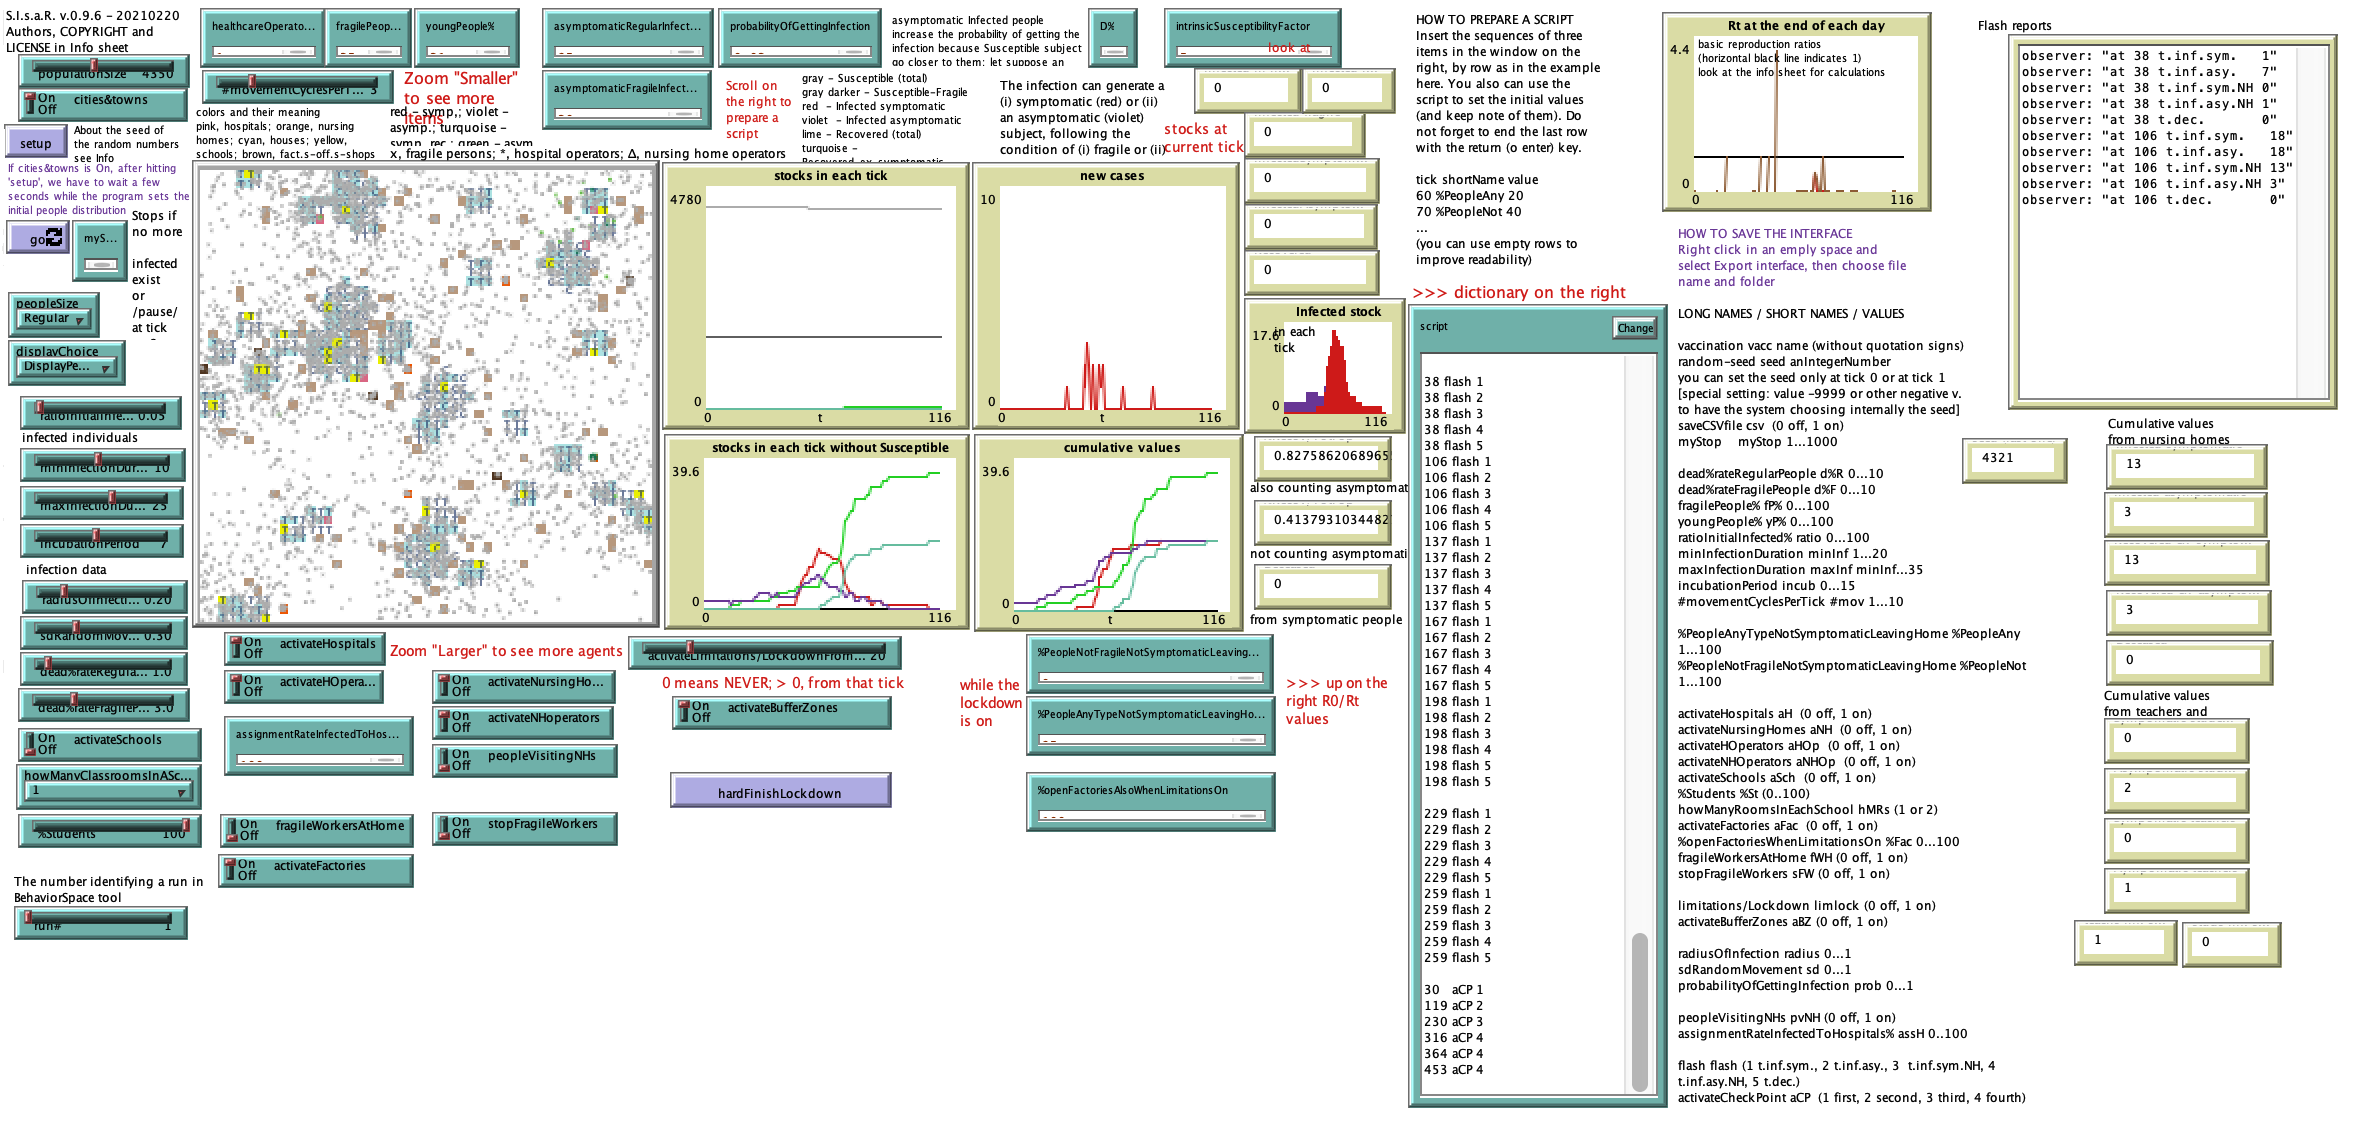
\includegraphics[scale=0.14]{interface2021.png}

%\caption{The interface} 
%\label{interface}
%\end{figure}

%\end{frame}

%%%%%%%%%%%%%%%%%%%%%%%%%%%%%%%%%%%%%%%%%%%%%%%%%%%%%%%%%
%\begin{frame}{The interface and the information sheet}

%\begin{figure}[H]
%\center
%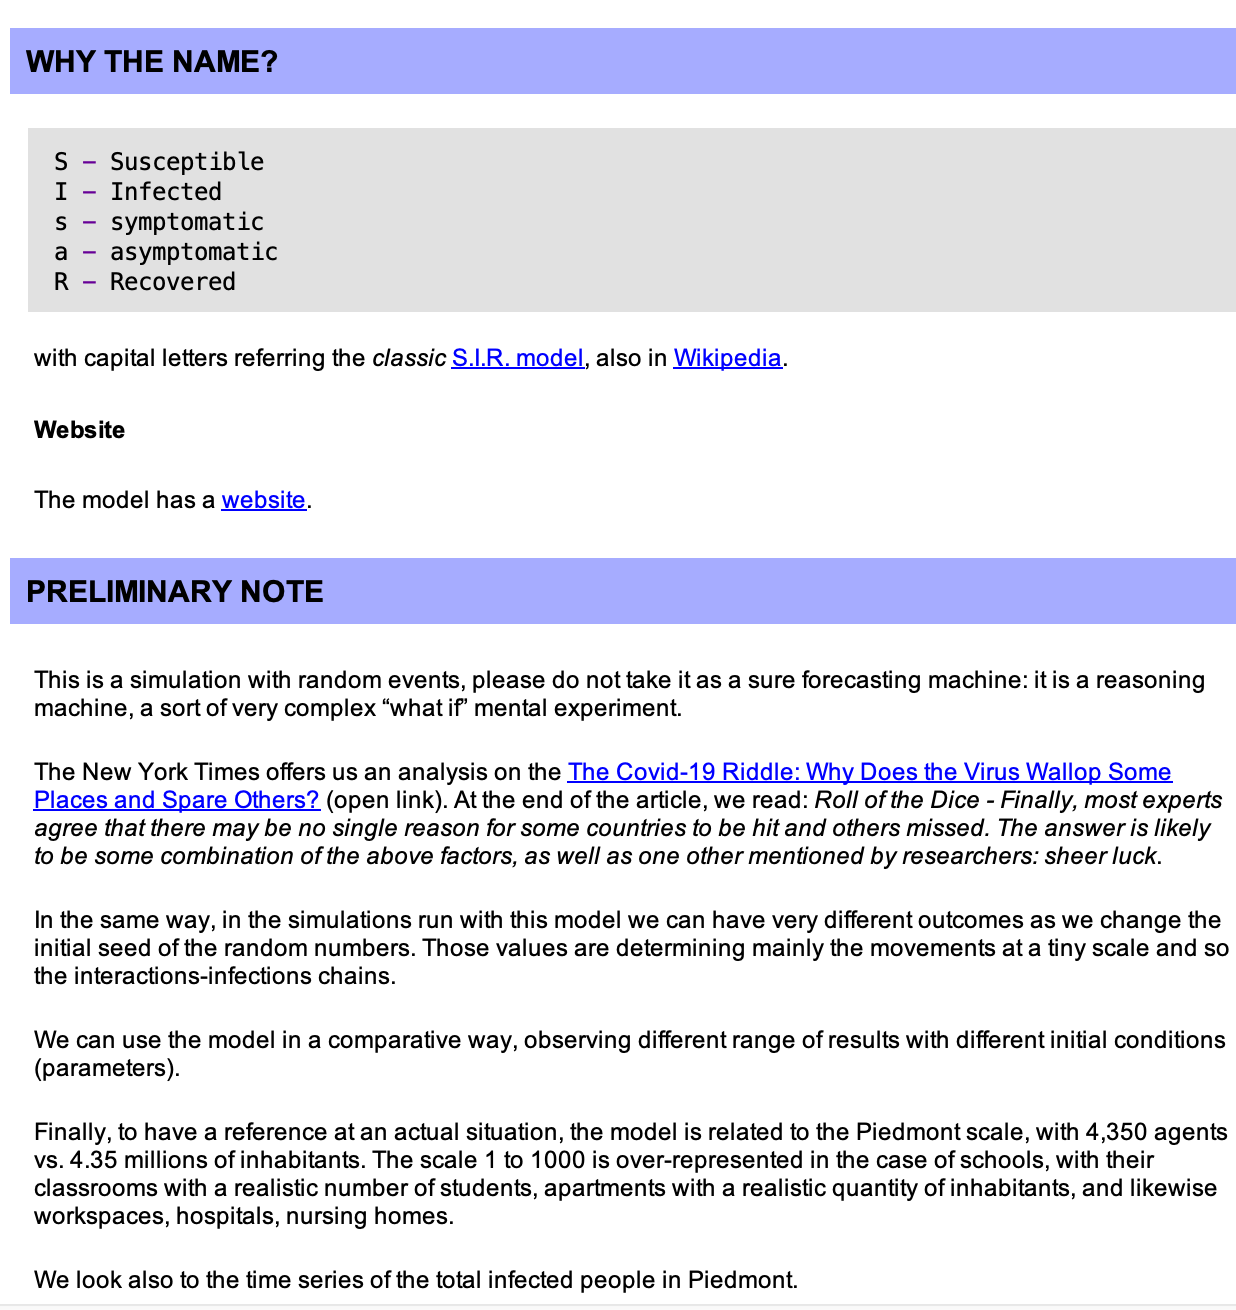
\includegraphics[scale=0.23]{info1b.png}~~~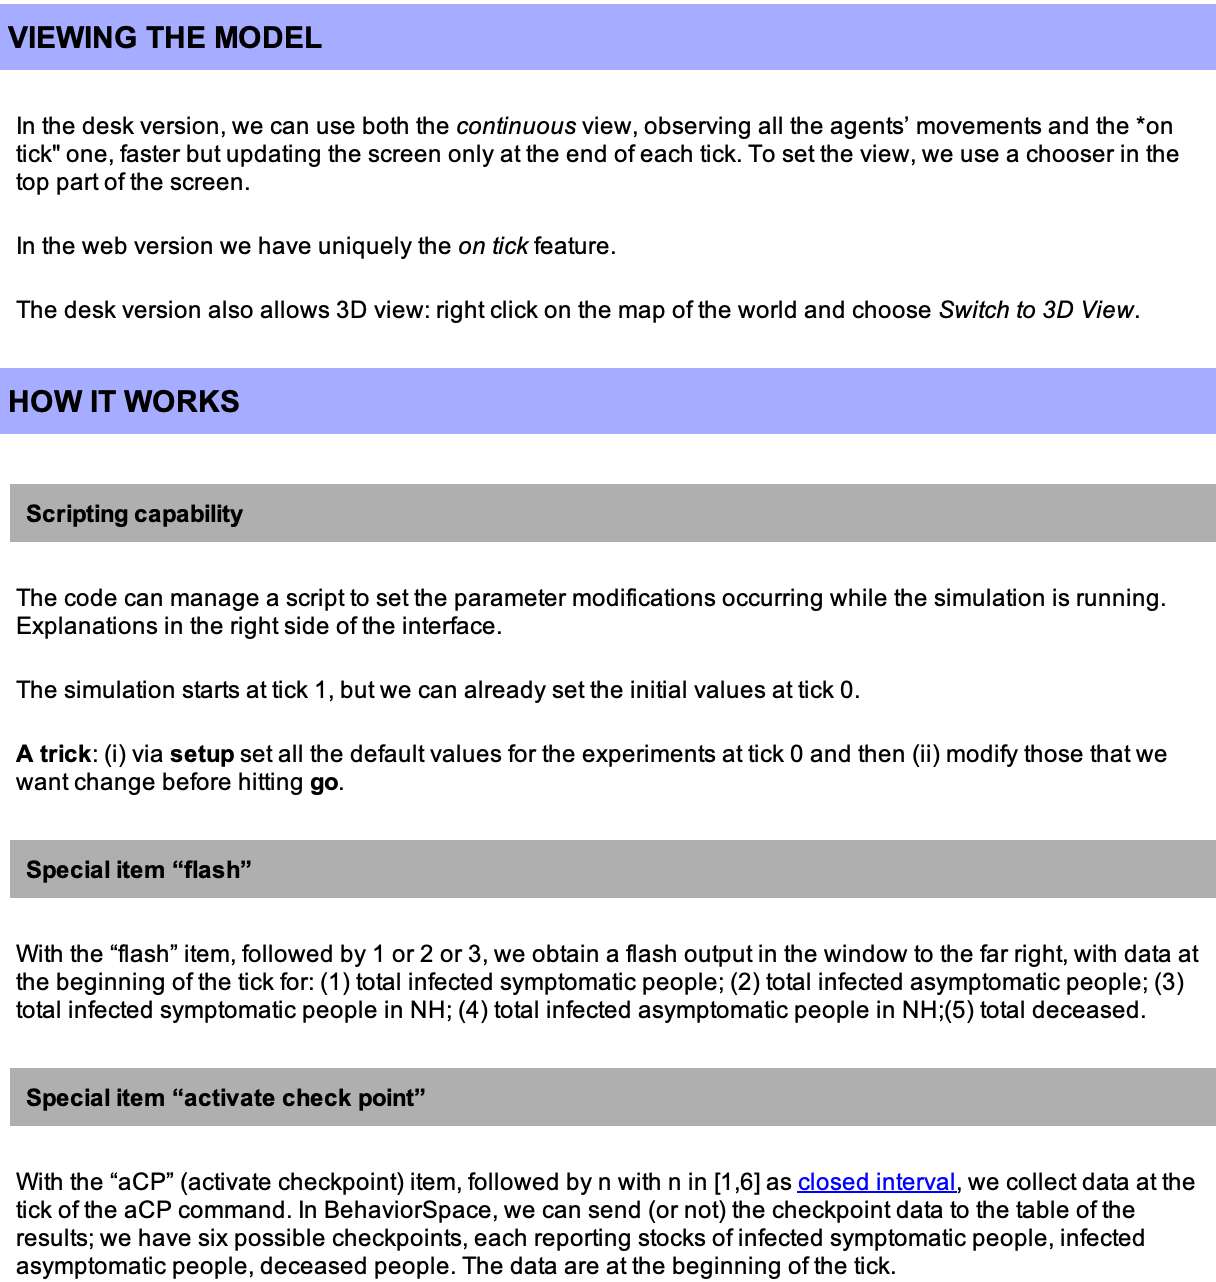
\includegraphics[scale=0.23]{info2b.png}

%\caption{The information sheet, about  20 pages} 
%\label{interface}
%\end{figure}

%\end{frame}

%%%%%%%%%%%%%%%%%%%%%%%%%%%%%%%%%%%%%%%%%%%%%%%%%%%%%%%%%
%\begin{frame}{The world}

%\begin{figure}[H]
%\center
%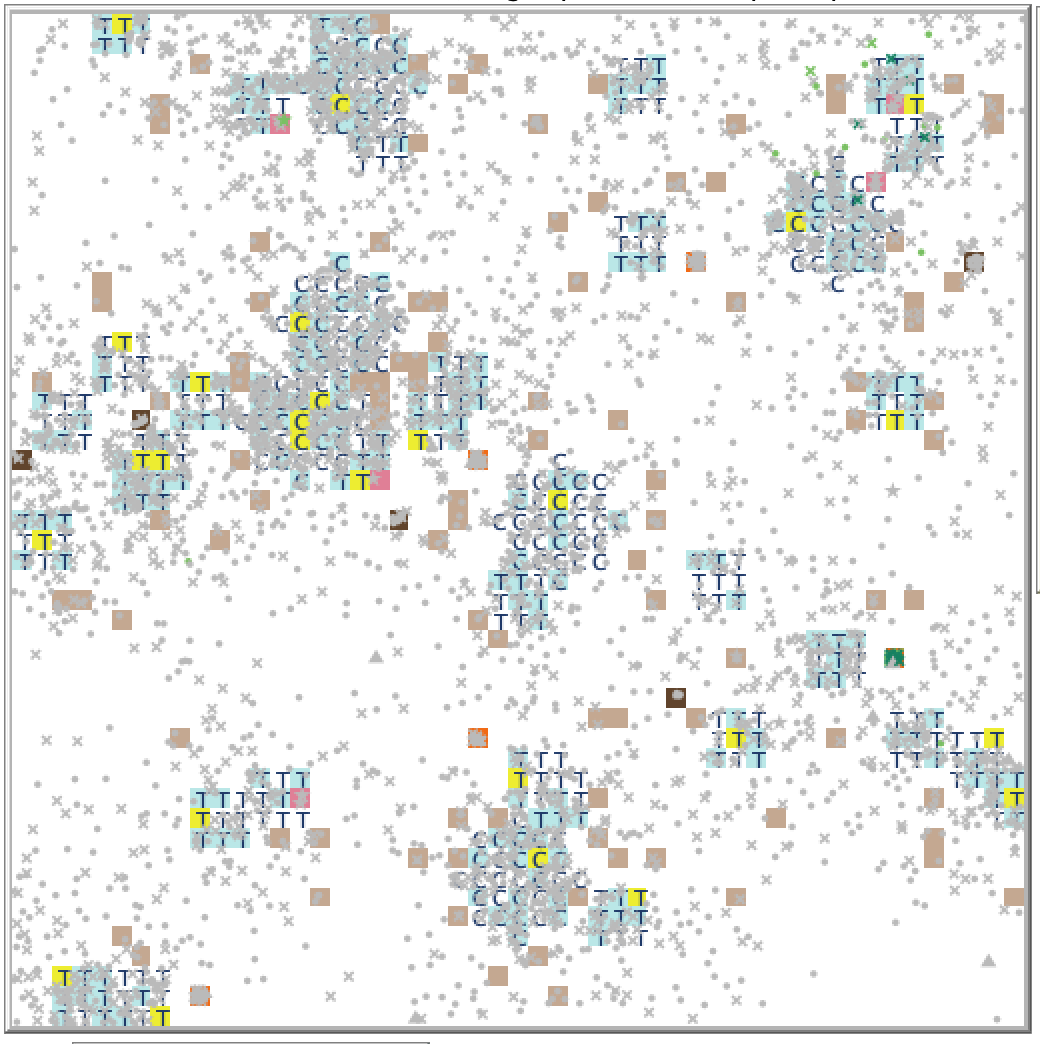
\includegraphics[scale=0.35]{world.png}

%\caption{The world} 
%\label{world}
%\end{figure}

%\end{frame}

%%%%%%%%%%%%%%%%%%%%%%%%%%%%%%%%%%%%%%%%%%%%%%%%%%%%%%%%%
\begin{frame}{The world 3D}

\begin{figure}[H]
\center
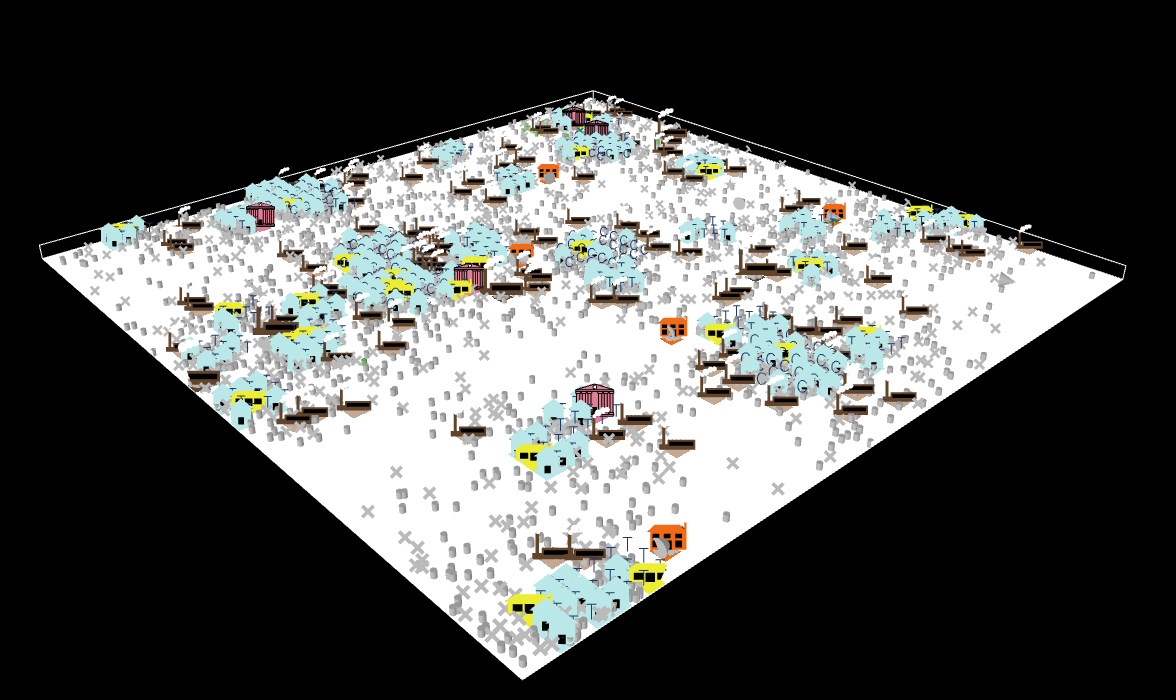
\includegraphics[scale=0.55]{world3D.png}

\caption{The world 3D} 
\label{world3D}
\end{figure}

\end{frame}

%%%%%%%%%%%%%%%%%%%%%%%%%%%%%%%%%%%%%%%%%%%%%%%%%%%%%%%%%
%\begin{frame}{The agents}

%\begin{figure}[H]
%\center
%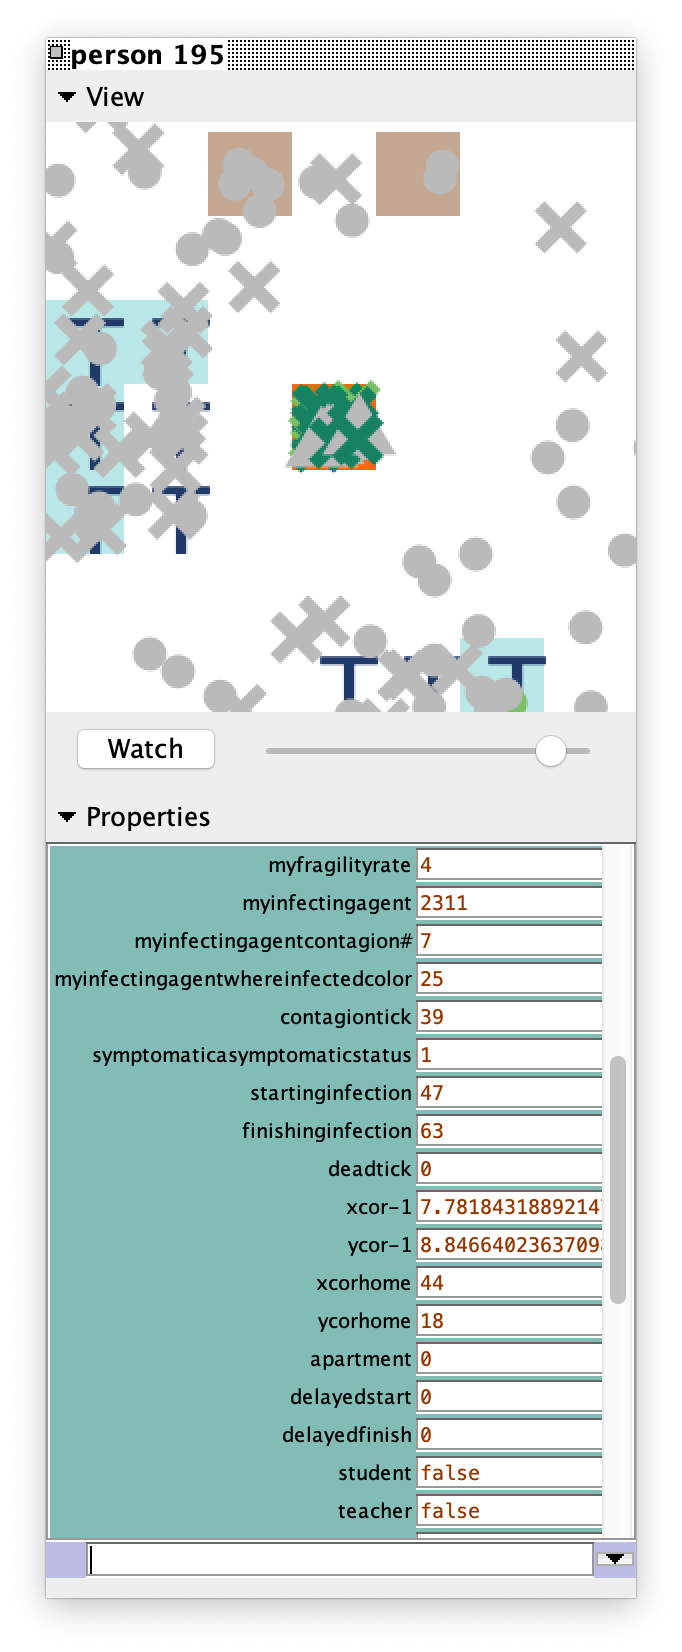
\includegraphics[scale=0.23]{person1.png}~~~~~~~~~~~~~~~~~~~~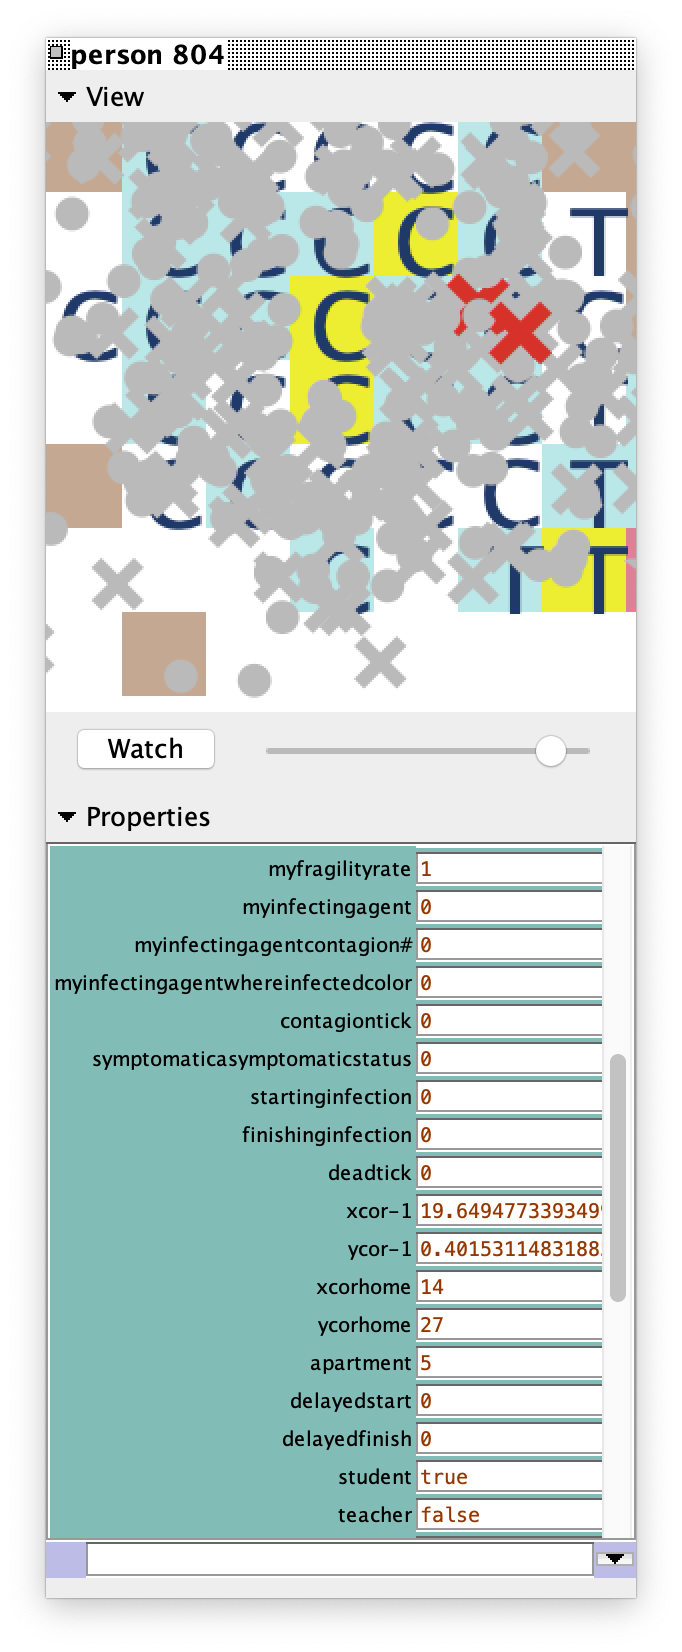
\includegraphics[scale=0.23]{person2.png}

%\caption{Probes to different agents} 
%\label{diffAgents}
%\end{figure}

%\end{frame}

%%%%%%%%%%%%%%%%%%%%%%%%%%%%%%%%%%%%%%%%%%%%%%%%%%%%%%%%%
\section{How the model works}

%%%%%%%%%%%%%%%%%%%%%%%%%%%%%%%%%%%%%%%%%%%%%%%%%%%%%%%%%
\subsection{A circular scheme}

%%%%%%%%%%%%%%%%%%%%%%%%%%%%%%%%%%%%%%%%%%%%%%%%%%%%%%%%%
\begin{frame}{A circular scheme}

\begin{figure}[H]
\center
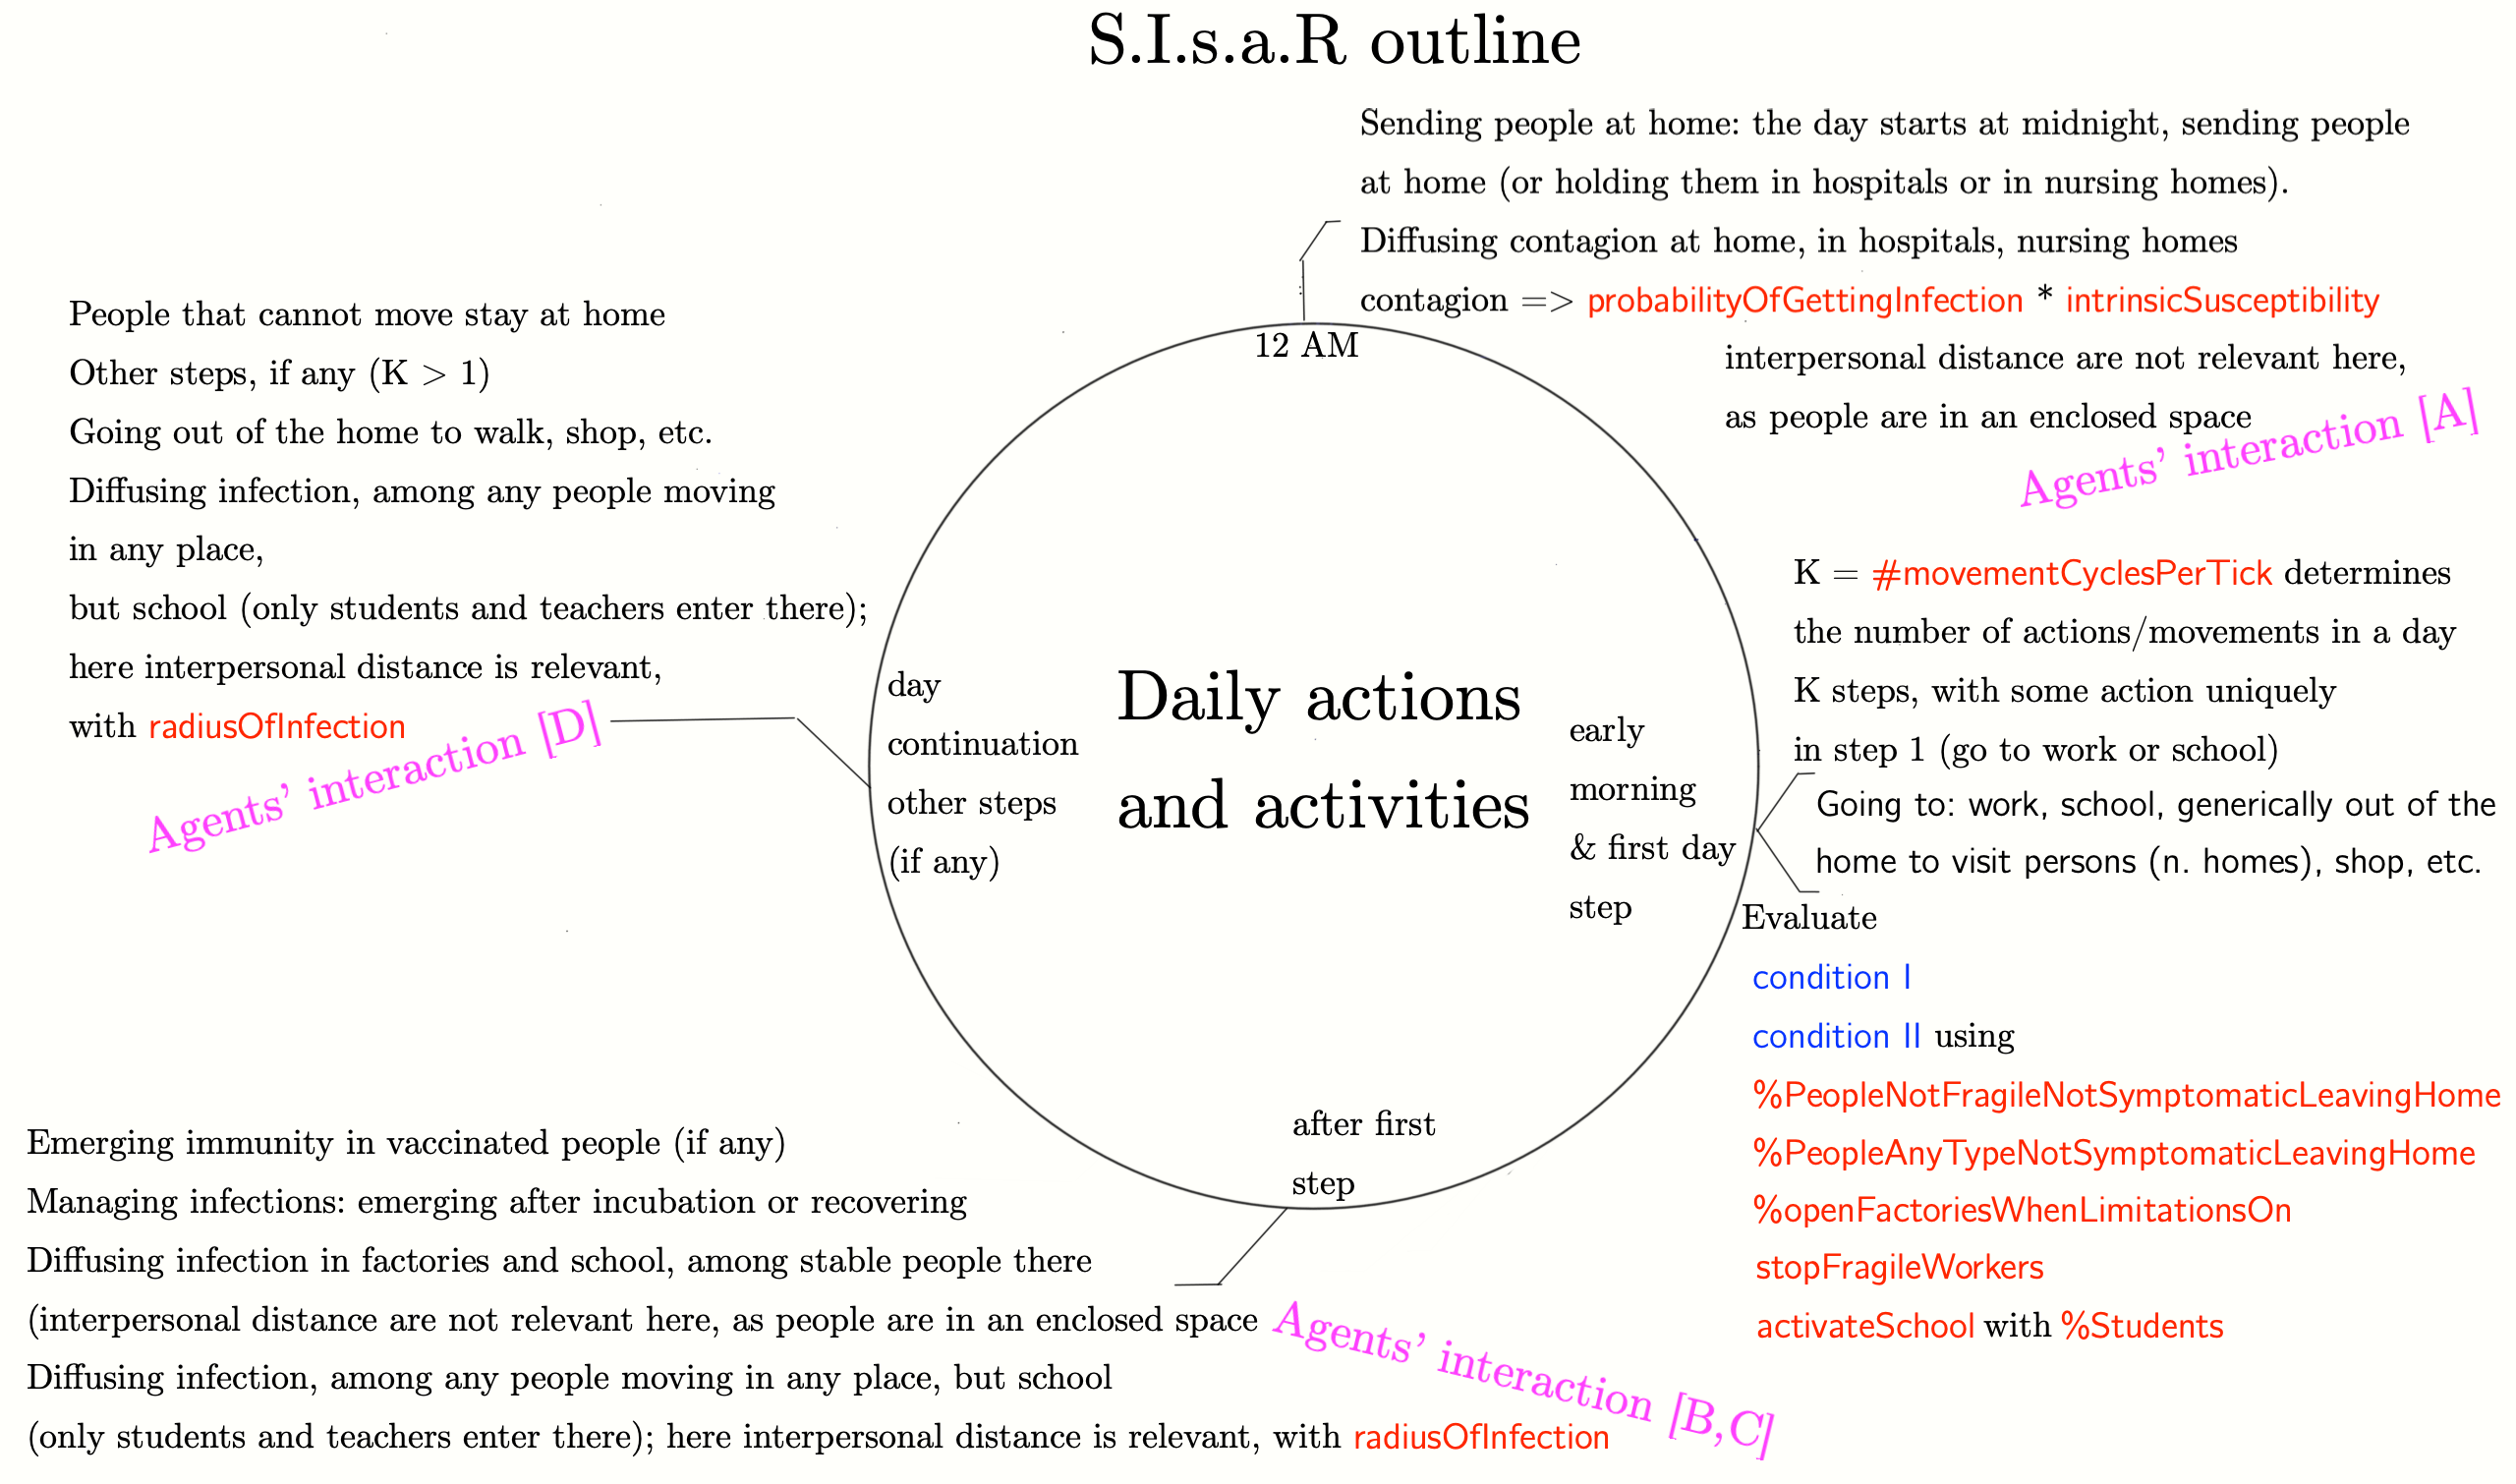
\includegraphics[scale=0.12]{SIsaR_outline.png}

\caption{The scheme: def. and values of the parameters at \url{https://terna.to.it/simul/howSIsaRworks.pdf}} 
\label{SIsaR_outline}
\end{figure}

\end{frame}

%%%%%%%%%%%%%%%%%%%%%%%%%%%%%%%%%%%%%%%%%%%%%%%%%%%%%%%%%
\subsection{Contagion representation}

%%%%%%%%%%%%%%%%%%%%%%%%%%%%%%%%%%%%%%%%%%%%%%%%%%%%%%%%%
\begin{frame}{Contagion representation}

  \begin{itemize}
  \item
The model allows analyzing the sequences of contagions in simulated epidemics, reporting the places where the contagion occur. 
  \item
We represent each infected agent as a horizontal segment (from the starting date to the final date of the infection) with vertical connections to other agents if they receive the disease.

We represent the new infected agents via further segments at an upper level. 

  \item
With colors, line thickness, and styles, we display multiple information. 

  \item
This enables understanding at a glance how an epidemic episode is developing. In this way, it is easier to reason about countermeasures and, thus, to develop intervention policies.

  \end{itemize}
\end{frame}


%%%%%%%%%%%%%%%%%%%%%%%%%%%%%%%%%%%%%%%%%%%%%%%%%%%%%%%%%
\begin{frame}{Examples (1/2)}

\begin{figure}[H]
\center
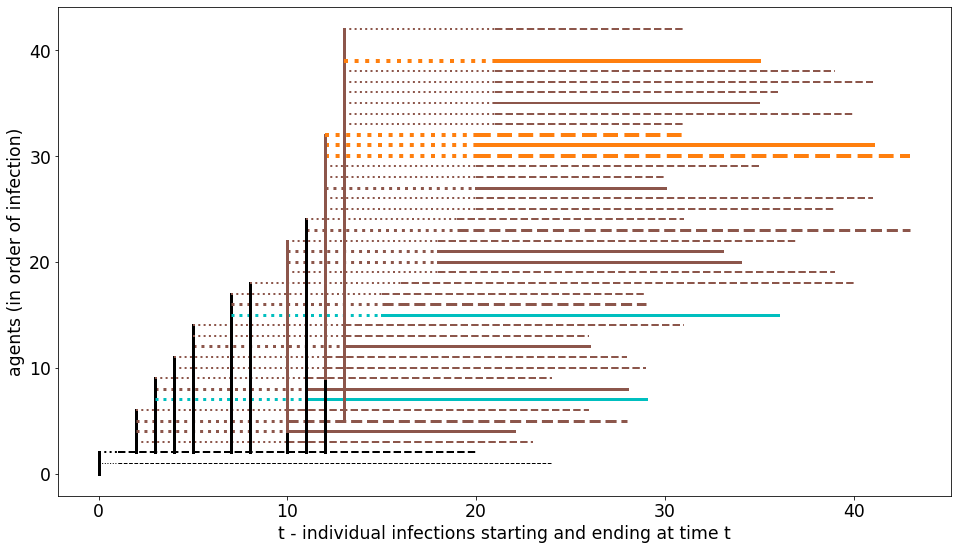
\includegraphics[width=0.9\textwidth]{with8b40.png}% with control case 473323 474697 in SIsaR_0.9.4.1 experiments 2 seeds with control-table_10000.csv, file withControl_473323_474697.csv
\caption{A case with containment measures, first 40 infections: workplaces (brown) and nursing homes (orange) strictly interweaving}
\label{workplacesNursingHomes}
\end{figure}
\end{frame}

%%%%%%%%%%%%%%%%%%%%%%%%%%%%%%%%%%%%%%%%%%%%%%%%%%%%%%%%%
\begin{frame}{Examples (2/2), whole epidemic}

\begin{figure}[H]
\center
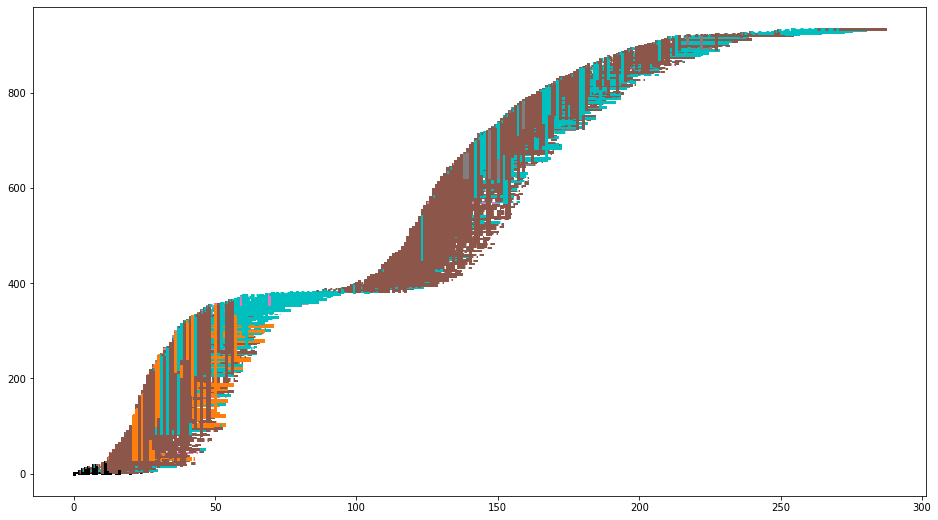
\includegraphics[width=0.9\textwidth]{with8a.png}% with control case 473323 474697 in SIsaR_0.9.4.1 experiments 2 seeds with control-table_10000.csv, file withControl_473323_474697.csv
\caption{A Case with containment measures, the whole epidemics: workplaces (brown) and nursing homes (orange) and then houses (cyan), with a bridge connecting two waves}
\label{workplacesNursingHomes}
\end{figure}


\end{frame}

%%%%%%%%%%%%%%%%%%%%%%%%%%%%%%%%%%%%%%%%%%%%%%%%%%%%%%%%%
\section{Exploring cases}

%%%%%%%%%%%%%%%%%%%%%%%%%%%%%%%%%%%%%%%%%%%%%%%%%%%%%%%%%
\subsection{Simulation batches}

%%%%%%%%%%%%%%%%%%%%%%%%%%%%%%%%%%%%%%%%%%%%%%%%%%%%%%%%%
\begin{frame}{Simulation batches}

  \begin{itemize}
  \item

We explore systematically the introduction of factual, counterfactual, and prospective interventions to control the spread of the contagions. 

  \item
Each simulation run---whose length corresponds to the disappearance of symptomatic or asymptomatic contagion cases---is a datum in a wide scenario of variability in time and effects.   
  
  \item
We need to represent compactly the results  emerging from batches of simulation repetitions, to compare the  consequences of the basic assumptions adopted for each specific batch.

 \item
Besides summarizing the results with the usual statistical indicators, we adopt the technique of the heat-maps.

\item
Each heat-map reports the duration of each simulated epidemic in the $x$ axis and the number of the symptomatic, asymptomatic, and deceased agents in the $y$ axis. The $z$ axis is represented by the colors, as in the logarithmic scale on the right of each picture. 

\item
In our batches we have 10,000 runs.

\end{itemize}
\end{frame}

%%%%%%%%%%%%%%%%%%%%%%%%%%%%%%%%%%%%%%%%%%%%%%%%%%%%%%%%%
\subsection{Epidemics without and with control}

%%%%%%%%%%%%%%%%%%%%%%%%%%%%%%%%%%%%%%%%%%%%%%%%%%%%%%%%%
\begin{frame}{10,000 epidemics without control in Piedmont}

% readRunResults10kStableSeedsCPoints_noControl_ChangingWorld_plusHMlog

\begin{table}[H]
\center
\tiny

\begin{tabular}{lrrr}
\toprule
{} &  symptomatic &  totalInfected\&Deceased &  duration \\
\midrule
count &     10000.00 &                10000.00 &  10000.00 \\
mean  &       969.46 &                 2500.45 &    303.10 \\
std   &       308.80 &                  802.88 &     93.50 \\
\bottomrule
\end{tabular}

\label{noCTab}
%\caption{a caption}
\end{table}

\begin{figure}[H]
\center
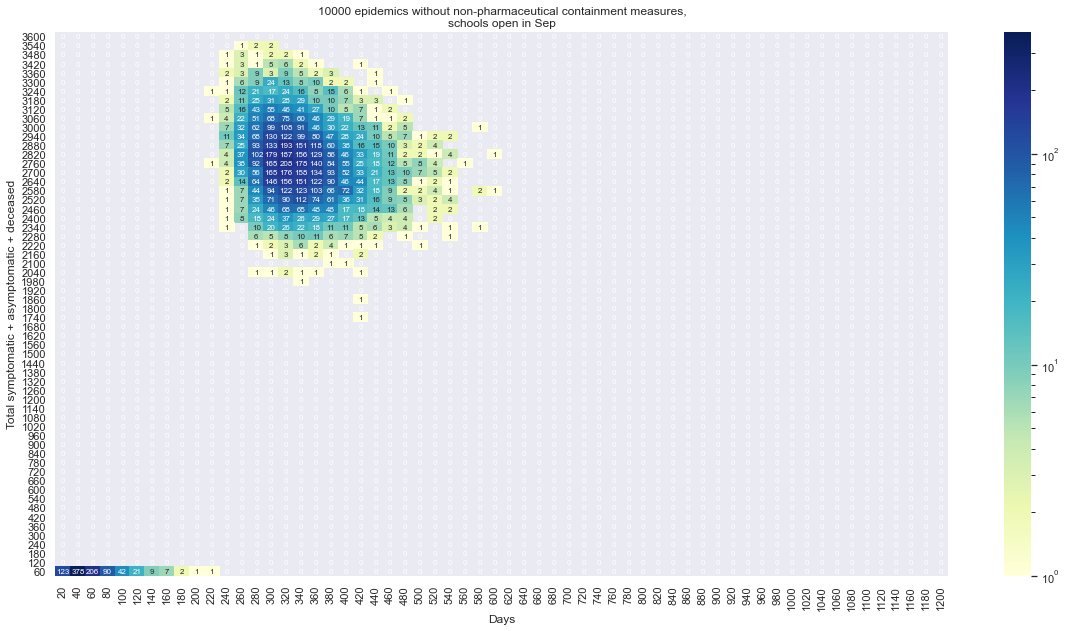
\includegraphics[scale=0.22]{10kNoControl.png}
\caption{Without non-pharmaceutical containment measures} 
\label{noC}
\end{figure}

\end{frame}


%%%%%%%%%%%%%%%%%%%%%%%%%%%%%%%%%%%%%%%%%%%%%%%%%%%%%%%%%
\begin{frame}{10,000 epidemic with basic control in Piedmont}

% readRunResults10kStableSeedsCPoints_basicControlB_schoolOpenSeptChangingWorld_plusHMlog

\begin{table}[H]
\center
\tiny

\begin{tabular}{lrrr}
\toprule
{} &  symptomatic &  totalInfected\&Deceased &  duration \\
\midrule
count &     10000.00 &                10000.00 &  10000.00 \\
mean  &       344.22 &                  851.64 &    277.93 \\
std   &       368.49 &                  916.41 &    213.48 \\
\bottomrule
\end{tabular}

\label{basicCTab}
%\caption{a caption}
\end{table}

\begin{figure}[H]
\center
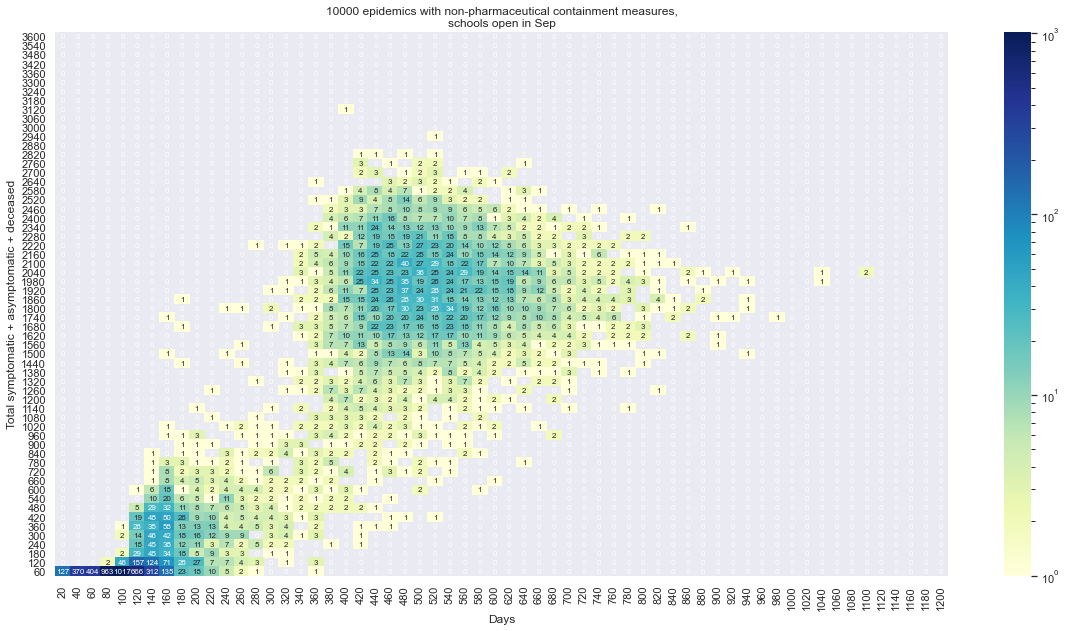
\includegraphics[scale=0.22]{10kBasicC.png}
\caption{First wave with non-pharmaceutical containment measures} 
\label{basicC}
\end{figure}

\end{frame}


%%%%%%%%%%%%%%%%%%%%%%%%%%%%%%%%%%%%%%%%%%%%%%%%%%%%%%%%%
\subsection{Actual data}

%%%%%%%%%%%%%%%%%%%%%%%%%%%%%%%%%%%%%%%%%%%%%%%%%%%%%%%%%
\begin{frame}{Key points (Summer and Fall 2020)}

\begin{figure}[H]
\center
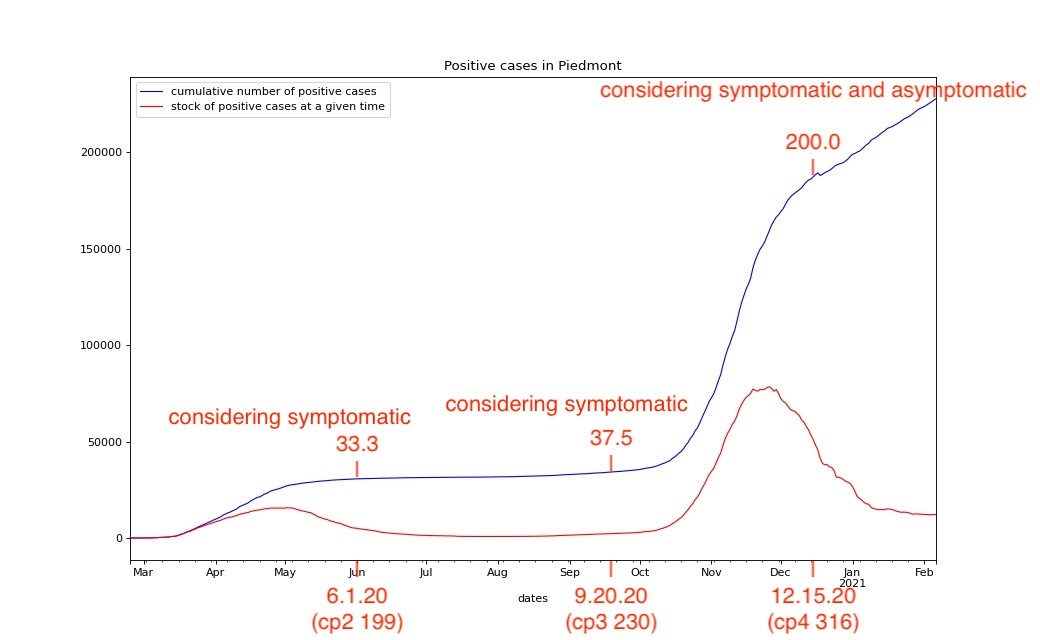
\includegraphics[scale=0.25]{andamento900annotato.jpg}
\caption{key points in epidemic dynamic in Summe and Fall 2020} 
\label{Key points}
\end{figure}


\end{frame}

%%%%%%%%%%%%%%%%%%%%%%%%%%%%%%%%%%%%%%%%%%%%%%%%%%%%%%%%%
\begin{frame}{Non homogeneous data}

\begin{itemize}

\item Following the Civil Protection Department web site \url{http://www.protezionecivile.it/web/guest/department}, we find the
 repository \url{https://github.com/pcm-dpc/COVID-19}.
 
 \item In the first wave we had uniquely data about symptomatic infected people, but from October 2020 data are mixed.
 
 \item In the above \emph{git}  repository, in October and November we had ``Positive cases emerged from clinical activity'', unfortunately then reported as ``No longer populated'' (from the end of November, my observation) and ``Positive cases emerging from surveys and tests, planned at national or regional level'', again ``No longer populated'' (from the end of November, my observation).
 
 \item Using those two series, it was possible to estimate a subdivision between symptomatic and asymptomatic cases, which is no longer possible.
 
\end{itemize}

\end{frame}




%%%%%%%%%%%%%%%%%%%%%%%%%%%%%%%%%%%%%%%%%%%%%%%%%%%%%%%%%
\begin{frame}{Updated series, with a third wave (data until the beginning of June)}

\begin{figure}[H]
\center
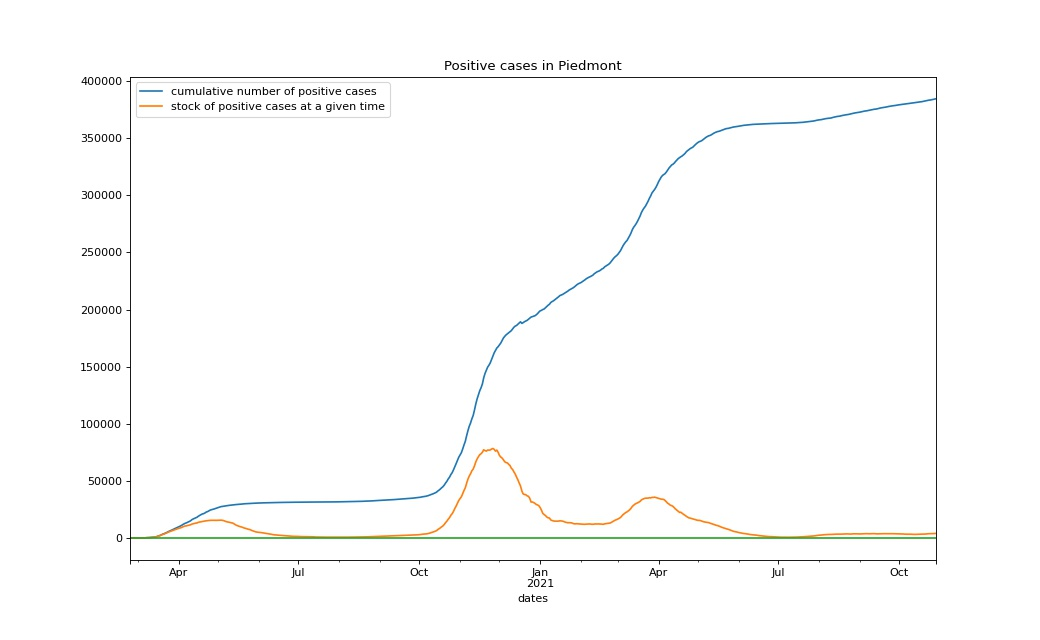
\includegraphics[scale=0.35]{andamento900AA.jpg}
\caption{Data for Piedmont} 
\label{dataP}
\end{figure}


\end{frame}




%%%%%%%%%%%%%%%%%%%%%%%%%%%%%%%%%%%%%%%%%%%%%%%%%%%%%%%%%
\section{Factual/counterfactual analyses}

%1%%%%%%%%%%%%%%%%%%%%%%%%%%%%%%%%%%%%%%%%%%%%%%%%%%%%%%%%
\begin{frame}{Spontaneous second wave, without specific measures}

% selectResults10kStableSeedsCPoints_basicControlB_schoolOpenSeptChangingWorld_plusHMlog,ipynb
% using 10kCtrl1.csv from SIsaR_0.9.5.4.1trials10kCtrl1.nlogo

\textbf{170} {\tiny epidemics stable in Summer 2020 out of 10,000, rule: at Jun~1,~20 select if sym. (10, 70], actual v. 33.3 \& at Sep~20,~20 select if sym. (20, 90], actual value 37.5;} \textbf{140} {\tiny at Dec~15,~20, rule: sym.+asym.>Sep~20,~20, actual value: 200.0.}

\begin{figure}[H]
\center
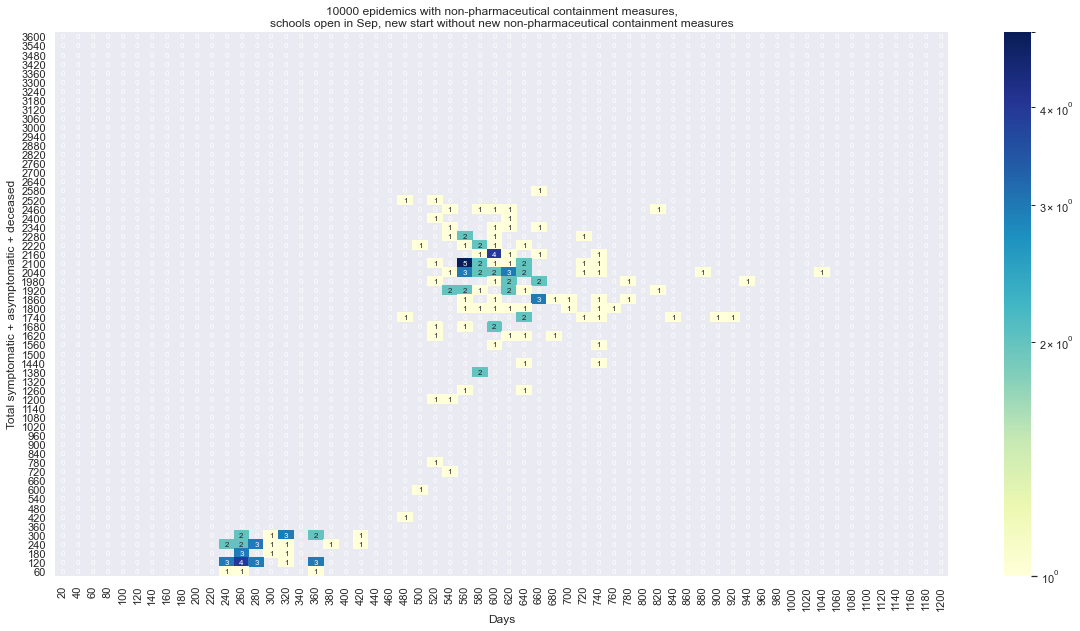
\includegraphics[scale=0.17]{10kSpontWave2.png}
\caption{First wave with non-pharmaceutical containment measures, spontaneous second wave, without specific measures}
\label{selSpontWave2}
\end{figure}

%\vspace{-0.4cm}

\begin{table}[H]
\center
\tiny
\begin{tabular}{p{0.4cm}p{0.3cm}p{0.3cm}p{0.3cm}p{0.3cm}p{0.3cm}p{0.3cm}p{0.3cm}p{0.3cm}p{0.3cm}p{0.3cm}p{0.3cm}p{0.3cm}p{0.4cm}}
\toprule
(1000) &  Jun~1,~20 & &  Sep~9,~20 & & Dec~15,~20 & & Feb~1,~21 & & May~1,~21 & & Dec~15,~20~~~to~~~end  \\
cum.~v. &  sym. &  all &  sympt. &  totalInf. &  sympt. &  totalInf. &  sympt. &  totalInf. &  sympt. &  totalInf. &  sympt. &  totalInf.  & days\\
\midrule
count &    170.0 &                      170.0 &    170.0 &                      170.0 &    140.0 &                      140.0 &    131.0 &                      131.0 &    128.0 &                      128.0 &               140.0 &                   140.0 &  140.0 \\
mean  &     37.9 &                      100.2 &     60.4 &                      159.3 &    \textbf{248.4} &                      \textbf{648.7} &    \textbf{432.2} &                     \textbf{1109.5} &   \textbf{656.3} &                     \textbf{1655.5} &              701.1 &                  1757.9 &  594.2 \\
std   &     16.4 &                       61.0 &     19.6 &                       71.7 &    167.4 &                      424.3 &    220.4 &                      538.4 &    215.4 &                      513.3 &               246.4 &                   599.7 &  118.9 \\
\bottomrule
\end{tabular}

\label{selSpontWave2Tab}
%\caption{a caption}
\end{table}


\end{frame}

%2%%%%%%%%%%%%%%%%%%%%%%%%%%%%%%%%%%%%%%%%%%%%%%%%%%%%%%%%
\begin{frame}{Second w., new infections from outside, without specific measures}

% selectResults10kStableSeedsCPoints_basicControlB_schoolOpenSeptChangingWorldNewStart_plusHMlog.ipynb
% using 10kCtrl1NStart.csv from SIsaR_0.9.5.4.1trials10kCtrl1NStart.nlogo

\textbf{1407} {\tiny epidemics stable in Summer 2020 out of 10,000, rule: at Jun~1,~20 select if sym. (10, 70], actual v. 33.3 \& at Sep~20,~20 select if sym. (20, 90], actual value 37.5;} \textbf{1044} {\tiny at Dec~15,~20, rule: sym.+asym.>Sep~20,~20, actual value: 200.0.}

\begin{figure}[H]
\center
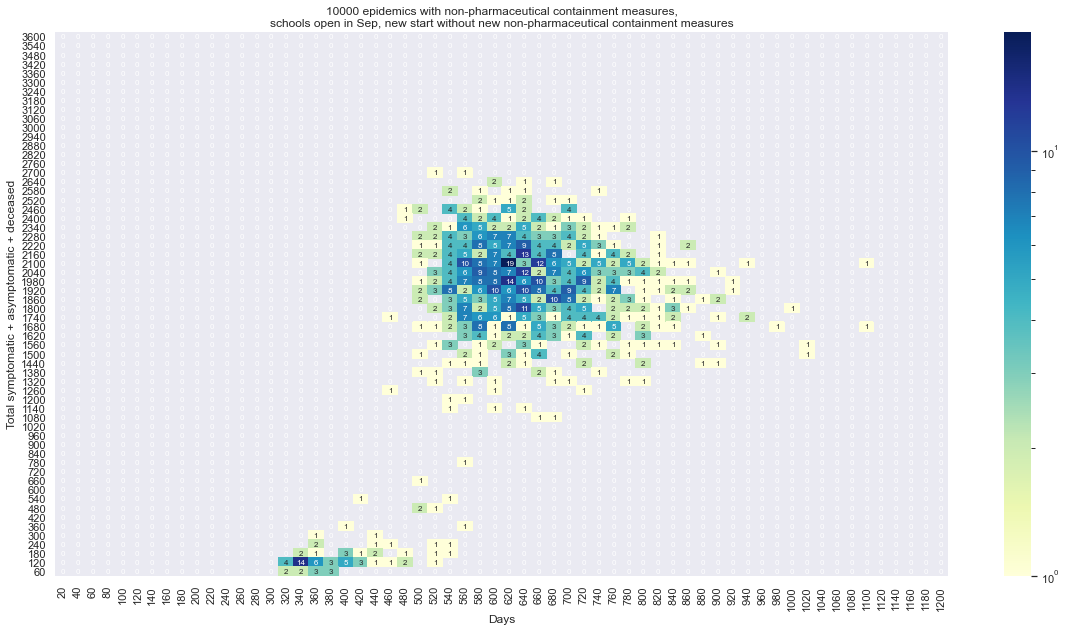
\includegraphics[scale=0.17]{10kForceWave2.png}
\caption{First wave with non-pharmaceutical containment measures, forcing the second wave, without specific measures}
\label{selForceWave2}
\end{figure}

%\vspace{-0.4cm}

\begin{table}[H]
\center
\tiny
\begin{tabular}{p{0.4cm}p{0.3cm}p{0.3cm}p{0.3cm}p{0.3cm}p{0.3cm}p{0.3cm}p{0.3cm}p{0.3cm}p{0.3cm}p{0.3cm}p{0.3cm}p{0.3cm}p{0.4cm}}
\toprule
(1000) &  Jun~1,~20 & &  Sep~9,~20 & & Dec~15,~20 & & Feb~1,~21 & & May~1,~21 & & Dec~15,~20~~~to~~~end   \\
cum.~v. &  sym. &  all &  sympt. &  totalInf. &  sympt. &  totalInf. &  sympt. &  totalInf. &  sympt. &  totalInf. &  sympt. &  totalInf.  & days\\
\midrule
count &   1407.0 &                     1407.0 &   1407.0 &                     1407.0 &   1044.0 &                     1044.0 &   1005.0 &                     1005.0 &    980.0 &                      980.0 &              1044.0 &                  1044.0 & 1044.0 \\
mean  &     35.6 &                       72.7 &     40.0 &                       84.1 &    \textbf{180.4} &                      \textbf{462.1} &    \textbf{354.1} &                      \textbf{900.4} &    \textbf{623.8} &                     \textbf{1563.3} &               726.6 &                  1810.9 &  620.9 \\
std   &     14.1 &                       42.6 &     16.7 &                       52.8 &    134.6 &                      354.6 &    213.8 &                      535.4 &    217.9 &                      527.0 &               221.9 &                   544.0 &  110.8 \\
\bottomrule
\end{tabular}

\label{selForceWave2Tab}
%\caption{a caption}
\end{table}


\end{frame}

%3%%%%%%%%%%%%%%%%%%%%%%%%%%%%%%%%%%%%%%%%%%%%%%%%%%%%%%%%
\begin{frame}{Second w., new infections from outside, with new specific measures}

% selectResults10kStableSeedsCPoints_basicControlB_schoolOpenSeptOctMarControlChangingWorldNewStart_plusHMlog.ipynb
% using 10kCtrl1NStartCtrl2M.csv from SIsaR_0.9.5.4.1trials10kCtrl1NStartCtrl2M.nlogo

\textbf{1407} {\tiny epidemics stable in Summer 2020 out of 10,000, rule: at Jun~1,~20 select if sym. (10, 70], actual v. 33.3 \& at Sep~20,~20 select if sym. (20, 90], actual value 37.5;} \textbf{874} {\tiny at Dec~15,~20, rule: sym.+asym.>Sep~20,~20, actual value: 200.0.}

\begin{figure}[H]
\center
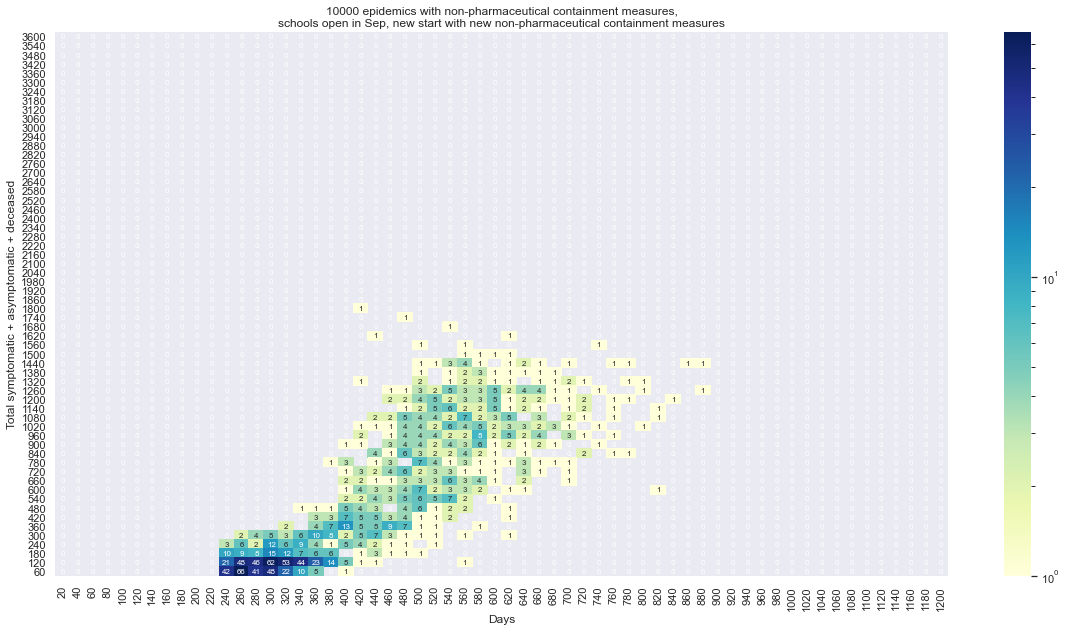
\includegraphics[scale=0.17]{10kForceWave2Contr2.png}
\caption{First wave with non-ph. containment measures, forcing the second wave, \textbf{with new specific non-ph. containment measures}}
\label{selForceWave2Contr2}
\end{figure}

%\vspace{-0.4cm}

\begin{table}[H]
\center
\tiny
\begin{tabular}{p{0.4cm}p{0.3cm}p{0.3cm}p{0.3cm}p{0.3cm}p{0.3cm}p{0.3cm}p{0.3cm}p{0.3cm}p{0.3cm}p{0.3cm}p{0.3cm}p{0.3cm}p{0.4cm}}
\toprule
(1000) &  Jun~1,~20 & &  Sep~9,~20 & & Dec~15,~20 & & Feb~1,~21 & & May~1,~21 & & Dec~15,~20~~~to~~~end   \\
cum.~v. &  sym. &  all &  sympt. &  totalInf. &  sympt. &  totalInf. &  sympt. &  totalInf. &  sympt. &  totalInf. &  sympt. &  totalInf.  & days\\
\midrule
count &   1407.0 &                     1407.0 &   1407.0 &                     1407.0 &    874.0 &                      874.0 &    719.0 &                      719.0 &    523.0 &                      523.0 &              874.0 &                   874.0 &  874.0 \\
mean  &     35.6 &                       72.7 &     40.0 &                       84.1 &    \textbf{130.0} &                      \textbf{340}.6 &    \textbf{194.4} &                      \textbf{512.8} &    \textbf{295.7} &                      \textbf{791.2} &               252.7 &                   666.4 &  494.1 \\
std   &     14.1 &                       42.6 &     16.7 &                       52.8 &     83.9 &                      232.6 &    104.1 &                      276.9 &    119.1 &                      300.6 &               156.8 &                   416.4 &  122.7 \\
\bottomrule
\end{tabular}

\label{selSpontWave2Contr2Tab}
%\caption{a caption}
\end{table}


\end{frame}

%%%%%%%%%%%%%%%%%%%%%%%%%%%%%%%%%%%%%%%%%%%%%%%%%%%%%%%%%
\begin{frame}{Time factor}

\begin{figure}[H]
\center
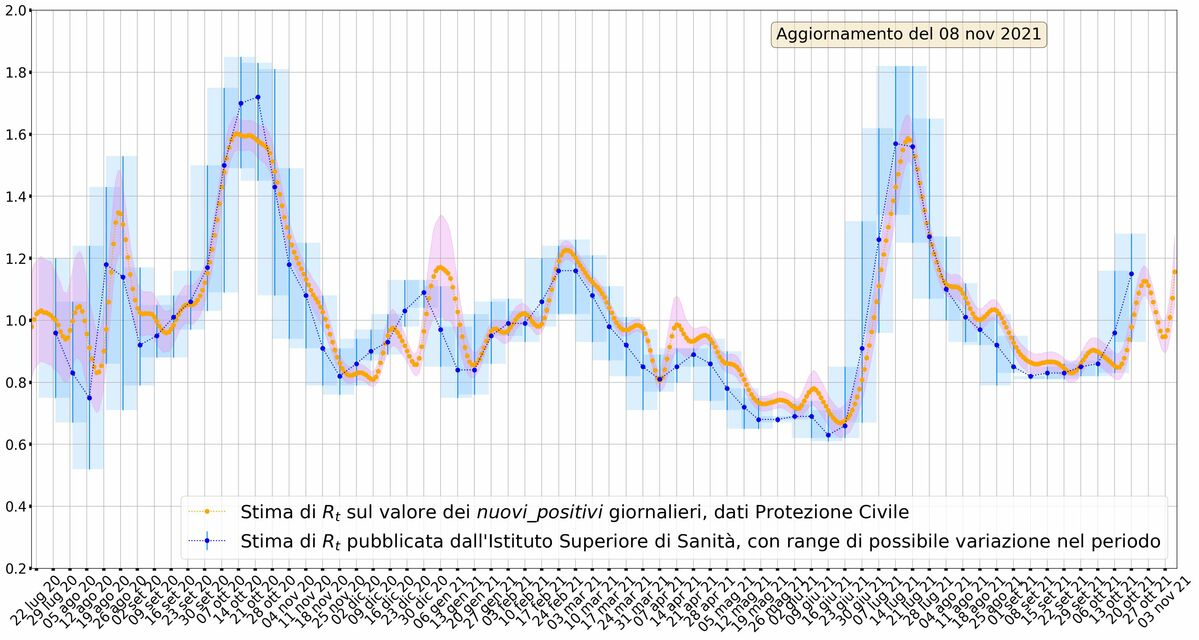
\includegraphics[scale=0.19]{RtEstimation4.jpg}
\caption{In blue the $R_t$ values as reported by the Istituto Superiore di Sanit\`{a} and in red the calculation published regularly at \url{https://mondoeconomico.eu} by Stefano Terna\footnote{Methodology: \url{https://github.com/tomorrowdata/COVID-19/blob/main/notebooks/Rt_on_italian_national_data.ipynb} and Section 5.4 at \url{https://arxiv.org/abs/2108.08885}}.}
\label{Rt}
\end{figure}


\end{frame}

%4%%%%%%%%%%%%%%%%%%%%%%%%%%%%%%%%%%%%%%%%%%%%%%%%%%%%%%%%
\begin{frame}{Second w., new infect. from outside, with new specific meas. -20 days\footnote{N.B.: (i) anticipation limit Oct 5.; (ii) also the ending date of each measure is anticipated of 20 days.}}

% selectResults10kStableSeedsCPoints_basicControlB_schoolOpenSeptOctMar-20ControlChangingWorldNewStart_plusHMlog.ipynb
% using 10kCtrl1NStartCtrl2M-20.csv from SIsaR_0.9.5.4.1trials10kCtrl1NStartCtrl2M-20.nlogo

\textbf{1407} {\tiny epidemics stable in Summer 2020 out of 10,000, rule: at Jun~1,~20 select if sym. (10, 70], actual v. 33.3 \& at Sep~20,~20 select if sym. (20, 90], actual value 37.5;} \textbf{769} {\tiny at Dec~15,~20, rule: sym.+asym.>Sep~20,~20, actual value: 200.0.}

\begin{figure}[H]
\center
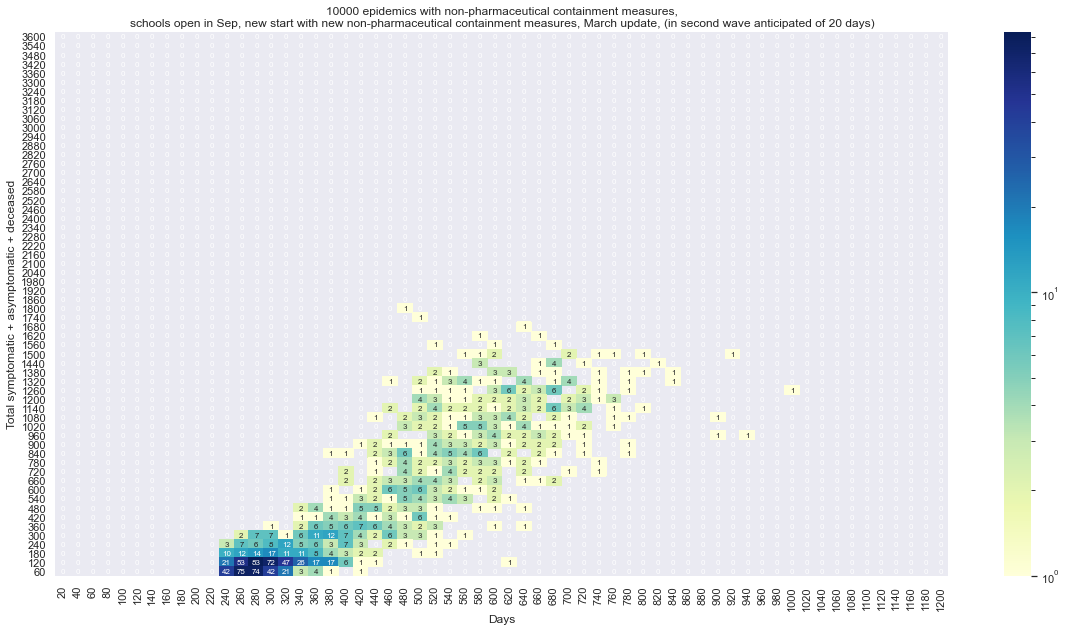
\includegraphics[scale=0.17]{10kForceWave2Contr2M-20.png}
\caption{First wave with non-ph. cont. meas., forcing the second wave, \textbf{with new specific non-ph. cont. meas., 20 day anticipation}}
\label{selForceWave2Contr2M-20}
\end{figure}

%\vspace{-0.4cm}

\begin{table}[H]
\center
\tiny
\begin{tabular}{p{0.4cm}p{0.3cm}p{0.3cm}p{0.3cm}p{0.3cm}p{0.3cm}p{0.3cm}p{0.3cm}p{0.3cm}p{0.3cm}p{0.3cm}p{0.3cm}p{0.3cm}p{0.4cm}}
\toprule
(1000) &  Jun~1,~20 & &  Sep~9,~20 & & Dec~15,~20 & & Feb~1,~21 & & May~1,~21 & & Dec~15,~20~~~to~~~end   \\
cum.~v. &  sym. &  all &  sympt. &  totalInf. &  sympt. &  totalInf. &  sympt. &  totalInf. &  sympt. &  totalInf. &  sympt. &  totalInf.  & days\\
\midrule
count &   1407.0 &                     1407.0 &   1407.0 &                     1407.0 &    769.0 &                      769.0 &    637.0 &                      637.0 &    471.0 &                      471.0 &              769.0 &                   769.0 &  769.0 \\
mean  &     35.6 &                       72.7 &     40.0 &                       84.1 &    \textbf{{\color{red}112.2}} &                     \textbf{{\color{red} 294.2}} &    \textbf{172.0} &                      \textbf{467.9} &    \textbf{276.5} &                      \textbf{748.6} &              248.9 &                   663.4 &  499.3 \\
std   &     14.1 &                       42.6 &     16.7 &                       52.8 &     66.8 &                      188.4 &     91.5 &                      251.3 &    112.9 &                      286.9 &               158.0 &                   417.5 &  124.1 \\
\bottomrule
\end{tabular}

\label{selForceWave2Contr2M-20Tab}
%\caption{a caption}
\end{table}


\end{frame}

%%%%%%%%%%%%%%%%%%%%%%%%%%%%%%%%%%%%%%%%%%%%%%%%%%%%%%%%%
\begin{frame}{Fragile persons}

\begin{itemize}


\item
A possible strategy is to stop all fragile people for a given period when $R_t$ starts increasing (also with fragile workers in sick leave, if unable to work remotely).

\item
We have also relevant social benefits, e.g., schooling, and economic benefits, as activities do not stop


\end{itemize}

\end{frame}



%5%%%%%%%%%%%%%%%%%%%%%%%%%%%%%%%%%%%%%%%%%%%%%%%%%%%%%%%%
\begin{frame}{Sec. w., new infect. from outs., stop fragile people. 60  days from Oct. 5\footnote{Schools are always working 100\% in this case.}}

%selectResults10kStableSeedsCPoints_basicControlB_schoolOpenSeptNoFragOCT05-60dControlChangingWorldNewStart_plusHMlog.ipynb
% using 10kCtrl1NStartNoFragOCT05-60d.csv from SIsaR_0.9.5.4.1trials10kCtrl1NStartNoFragOCT05-60d.nlogo

\textbf{1407} {\tiny epidemics stable in Summer 2020 out of 10,000, rule: at Jun~1,~20 select if sym. (10, 70], actual v. 33.3 \& at Sep~20,~20 select if sym. (20, 90], actual value 37.5;} \textbf{886} {\tiny at Dec~15,~20, rule: sym.+asym.>Sep~20,~20, actual value: 200.0.}

\begin{figure}[H]
\center
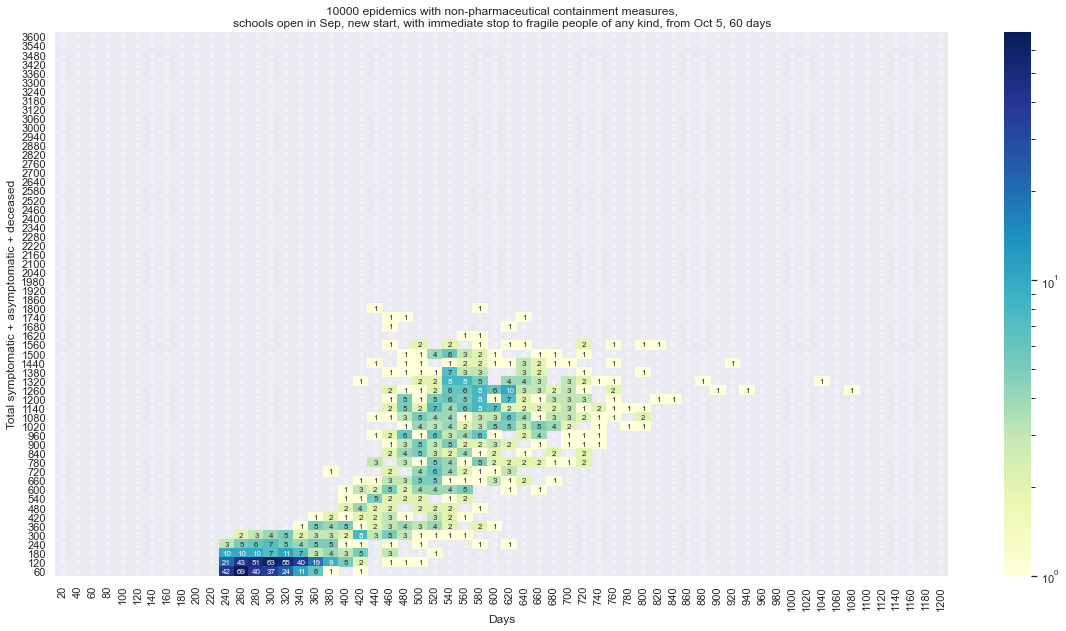
\includegraphics[scale=0.17]{10kForceWave2NoFragOct5for60d.png}
\caption{First wave with non-ph. cont. meas., forcing the sec. w.; \textbf{in sec. w., uniquely stop fragile people, including fragile workers}} 
\label{selForceWave2NoFrag}
\end{figure}

%\vspace{-0.4cm} 

\begin{table}[H]
\center
\tiny
\begin{tabular}{p{0.3cm}p{0.3cm}p{0.3cm}p{0.3cm}p{0.3cm}p{0.3cm}p{0.3cm}p{0.3cm}p{0.3cm}p{0.3cm}p{0.3cm}p{0.3cm}p{0.3cm}p{0.4cm}}
\toprule
(1000) &  Jun~1,~20 & &  Sep~9,~20 & & Dec~15,~20 & & Feb~1,~21 & & May~1,~21 & & Dec~15,~20~~~to~~~end   \\
{} &  sym. &  all &  sympt. &  totalInf. &  sympt. &  totalInf. &  sympt. &  totalInf. &  sympt. &  totalInf. &  sympt. &  totalInf.  & days\\
\midrule
count &   1407.0 &                     1407.0 &   1407.0 &                     1407.0 &    886.0 &                      886.0 &    761.0 &                      761.0 &    637.0 &                      637.0 &              886.0 &                   886.0 &  886.0 \\
mean  &     35.6 &                       72.7 &     40.0 &                       84.1 &    \textbf{{\color{cyan}128.1}} &                      \textbf{{\color{cyan}326.3}} &    \textbf{211.0} &                      \textbf{555.1} &    \textbf{323.3} &                      \textbf{862.1} &               301.1 &                   792.3 &  515.5 \\
std   &     14.1 &                       42.6 &     16.7 &                       52.8 &     89.6 &                      234.2 &    118.1 &                      306.7 &    126.4 &                      315.9 &               170.7 &                   450.2 &  116.9 \\
\bottomrule
\end{tabular}

\label{selForceWave2NoFragTab}
%\caption{a caption}
\end{table}


\end{frame}




%%%%%%%%%%%%%%%%%%%%%%%%%%%%%%%%%%%%%%%%%%%%%%%%%%%%%%%%%
\begin{frame}{To recap (all waves)}

\begin{table}[H]
\center
\footnotesize
\begin{tabular}{p{1.8cm}p{0.5cm}p{0.5cm}p{0.5cm}p{0.5cm}p{0.5cm}p{0.5cm}}
\toprule
Scenarios     &    &  Dec~15,~20 &               & Dec~15,~20~~~to~~~end  &  &\\
                     &    & sympt.           &  totalInf. &  sympt. &  totalInf.  & days   \\                               

\midrule
no \\
containments in   & count & 140.0 &                      140.0 &                140.0 &                   140.0 &  140.0 \\
spontaneous         &  mean  &  \textbf{248.4} &                      \textbf{648.7} &      701.1 &                  1757.9 &  594.2 \\
second wave         & std  &  167.4 &                      424.3 &               246.4 &                   599.7 &  118.9 \\

\midrule
no \\
containments in   & count &     1044.0 &                     1044.0 &             1044.0 &                  1044.0 & 1044.0 \\
forced         & mean  &       \textbf{180.4} &                      \textbf{462.1} &          726.6 &                  1810.9 &  620.9 \\
second wave         & std   & 134.6 &                      354.6 &           221.9 &                   544.0 &  110.8 \\

\midrule
basic \\
containements in   & count &     874.0 &                      874.0 &          874.0 &                   874.0 &  874.0 \\
forced                    & mean  &             \textbf{130.0} &                      \textbf{340}.6 &                 252.7 &                   666.4 &  494.1 \\
second wave         & std   &   83.9 &                      232.6 &                  156.8 &                   416.4 &  122.7 \\
         
\midrule
-20 days \\ 
containments in   & count &  769.0 &                      769.0 &               769.0 &                   769.0 &  769.0 \\
forced             & mean  &   \textbf{{\color{red}112.2}} &        \textbf{{\color{red} 294.2}} &       248.9 &        663.4 &  499.3 \\
second wave  & std   &   66.8 &                      188.4 &          158.0 &                   417.5 &  124.1 \\

\midrule
frag. p. \& workers \\  
control in              & count &   886.0 &                      886.0 &              886.0 &                   886.0 &  886.0 \\
forced                  & mean  &  \textbf{{\color{cyan}128.1}} &         \textbf{{\color{cyan}326.3}} &          301.1 &        792.3 &  515.5 \\
second wave       & std   &  89.6 &        234.2 &   170.7 &          450.2 &  116.9 \\


\bottomrule
\end{tabular}
\caption{Report of the key results, with count, mean, and std}
\label{keyResultsT}
\end{table}



\end{frame}

%%%%%%%%%%%%%%%%%%%%%%%%%%%%%%%%%%%%%%%%%%%%%%%%%%%%%%%%%
\section{Planning vaccination campaigns}

%%%%%%%%%%%%%%%%%%%%%%%%%%%%%%%%%%%%%%%%%%%%%%%%%%%%%%%%%
\subsection{Introduction}

%%%%%%%%%%%%%%%%%%%%%%%%%%%%%%%%%%%%%%%%%%%%%%%%%%%%%%%%%
\begin{frame}{Planning a vaccination campaign using GAs (with non-pharmaceutical containment measures in action)}

\begin{itemize}

%\item An introduction to genetic algorithms (GAs) is at \url{https://en.wikipedia.org/wiki/Genetic_algorithm}, with the related Holland's schema theorem at 
%\url{https://en.wikipedia.org/wiki/Holland's_schema_theorem}.

\item Exploring vaccination sequences, using \emph{genetic algorithms}. A detailed note, frequently updated, is at \url{https://terna.to.it/simul/GAresultPresentation.pdf}.

\item We compare the effect of choosing the vaccination quotas via GAs with two predetermined strategies, considering three hypotheses (vaccinated people: still spread the contagion; do not spread the contagion; do it in the 50\% of the case); we show here only the first case results.

\item Key dates: 
\begin{itemize}
\item in the internal calendar of the model, day 373 is Feb. \nth{12}, 2021, which is effectively the starting point of the vaccinations in the region; 

\item the day of the effectiveness of the initial vaccinations, 40 days later, is day 413 (Mar. \nth{22}, 2021).
\end{itemize}

\end{itemize}

\end{frame}

%%%%%%%%%%%%%%%%%%%%%%%%%%%%%%%%%%%%%%%%%%%%%%%%%%%%%%%%%
\begin{frame}{Vaccination groups}

We take into consideration seven groups in order of decreasing fragility but also considering the exposure to contagion:

\begin{enumerate}
\item [\emph{g1}]
	extra fragile people with three components;
	\begin{itemize}
		\item due to intrinsic characteristics: people in nursing homes;
		\item due to risk exposure:
		\begin{itemize}
			\item nursing homes operators;
			\item healthcare operators;
 		\end{itemize} 
 	\end{itemize}  
\item [\emph{g2}]
	teachers;
\item [\emph{g3}]
	workers with medical fragility;
\item [\emph{g4}]
	regular workers;
\item [\emph{g5}]
	fragile people without special characteristics;
\item [\emph{g6}]
	regular people, not young, not worker, and not teacher;
\item [\emph{g7}]
	young people excluding special activity cases (a limited number in \emph{g1}).
\end{enumerate}

\end{frame}

%%%%%%%%%%%%%%%%%%%%%%%%%%%%%%%%%%%%%%%%%%%%%%%%%%%%%%%%%
\begin{frame}{A specific realistic case}

\begin{figure}[H]
\center
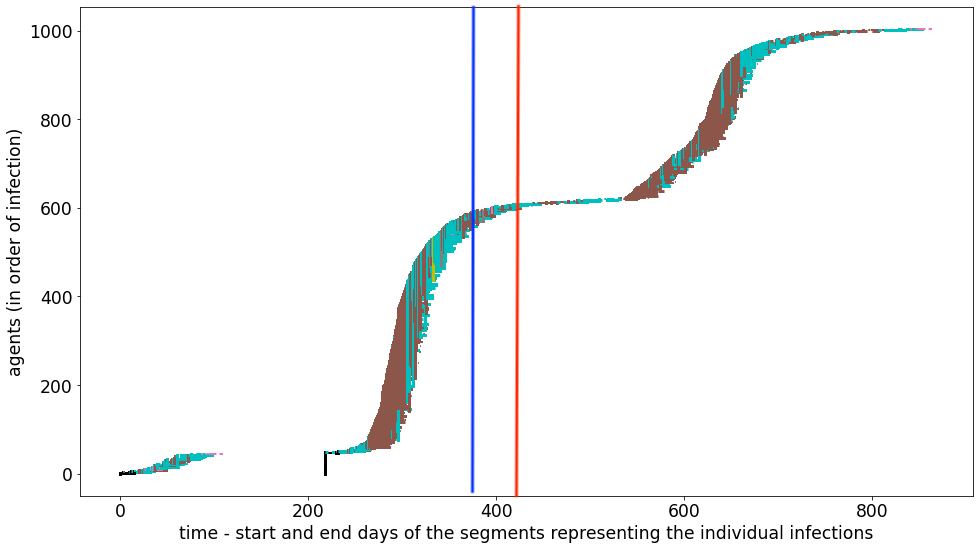
\includegraphics[scale=0.2]{CaseForGA_I_base.png}
\caption{Crucial dates: blue line for the starting point of the vaccination campaign and red line for the start of the effectiveness of the initial vaccinations}
\label{specificCase}
\end{figure}

\end{frame}

%%%%%%%%%%%%%%%%%%%%%%%%%%%%%%%%%%%%%%%%%%%%%%%%%%%%%%%%%
\subsection{An experiment with GA}

%%%%%%%%%%%%%%%%%%%%%%%%%%%%%%%%%%%%%%%%%%%%%%%%%%%%%%%%%
\begin{frame}{Time dynamics without vaccinations}

% using contagionSeriesByGroups.ipynb on Experiment_I_base.csv 
\begin{figure}[H]
\center
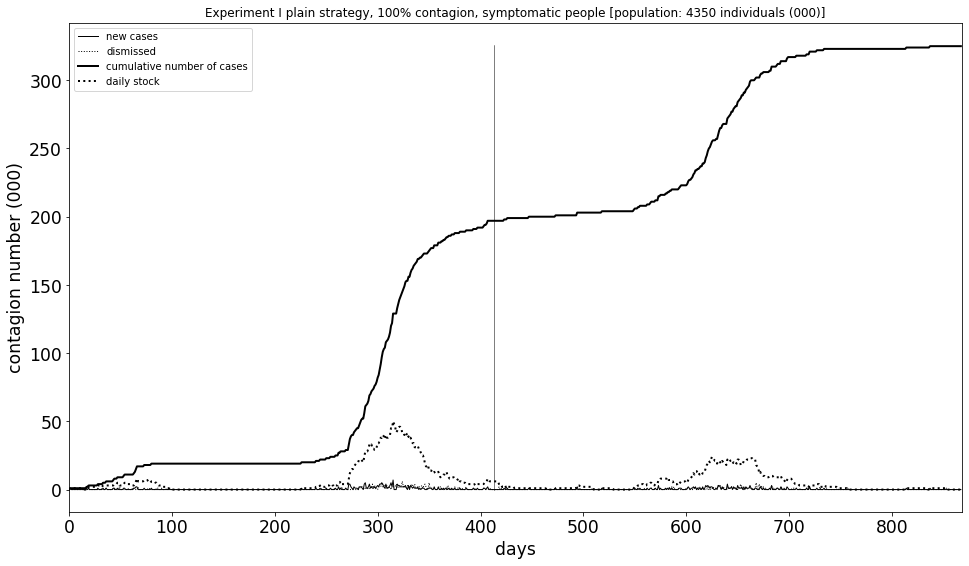
\includegraphics[scale=0.16]{Experiment_I_base_symptomatic_series.png} 

\caption{Experiment I, `base symptomatic series; the vertical line is at day 413 is not relevant here} 
\label{Experiment_I_plainSymptomaticSeries}
\end{figure}


\end{frame}

%%%%%%%%%%%%%%%%%%%%%%%%%%%%%%%%%%%%%%%%%%%%%%%%%%%%%%%%%

\begin{frame}{Time dynamics with \emph{plain} vac. strategy, vac. people still spreading the infection}

\begin{figure}[H]
\center
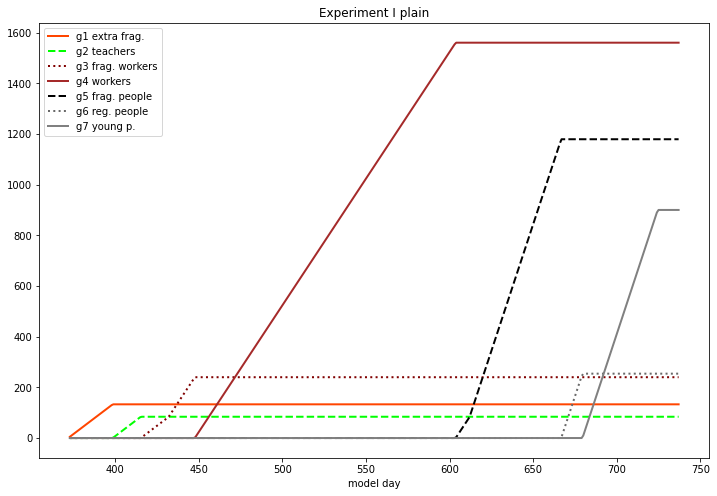
\includegraphics[scale=0.16]{Experiment_I_plainVaccinationSequence.png} % experiment_I_vaccination_plots.ipynb

\caption{``Plain'' vaccination sequence; on the $y$ axis the number of vaccinated subjects of each group (if vaccination is complete, the line is horizontal)} 
\label{Experiment_I_plainVaccinationSequence}
\end{figure}

% using contagionSeriesByGroups.ipynb on Experiment_I_plain_1.csv 
\begin{figure}[H]
\center
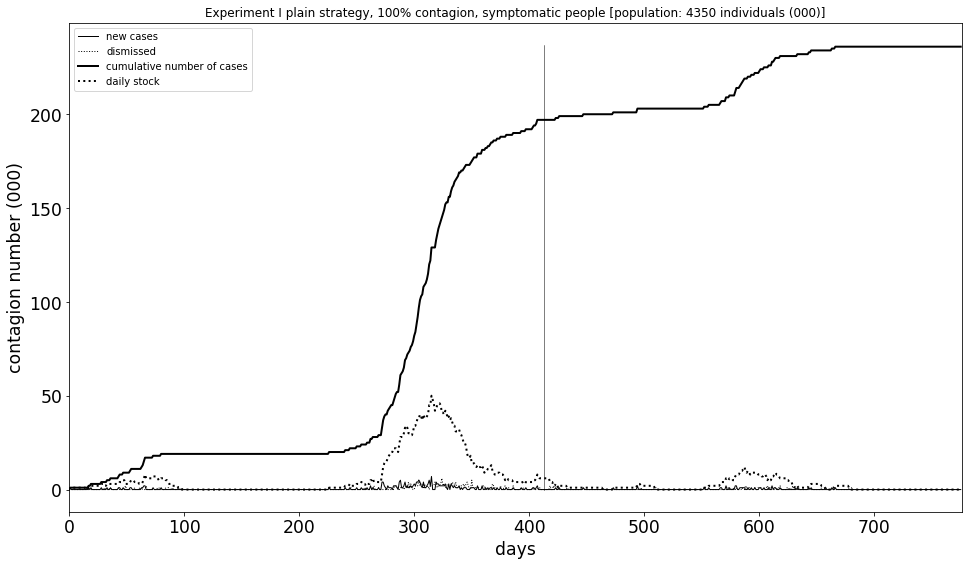
\includegraphics[scale=0.16]{Experiment_I_1_plain_symptomatic_series.png} 

\caption{``Plain'' vaccination symptomatic series; the vertical line is at day 413, when the effectiveness of first vaccination starts} 
\label{Experiment_I_plainSymptomaticSeries}
\end{figure}



\end{frame}

%%%%%%%%%%%%%%%%%%%%%%%%%%%%%%%%%%%%%%%%%%%%%%%%%%%%%%%%%
\begin{frame}{Time dynamics with \emph{wise} vac. strategy, vac. people still spreading the infection}

\begin{figure}[H]
\center
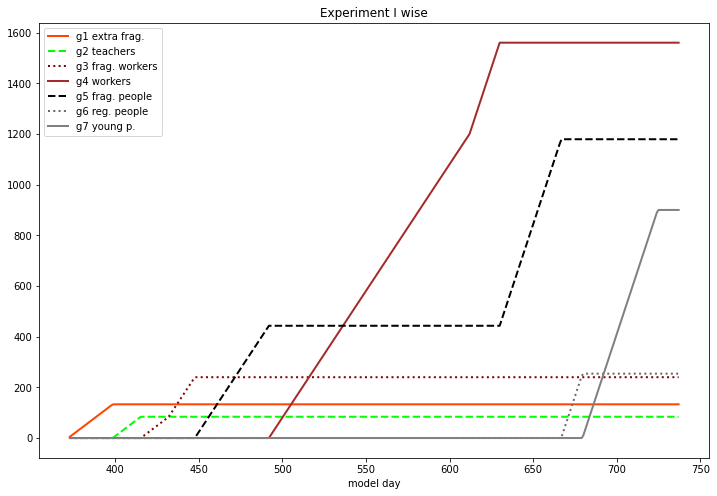
\includegraphics[scale=0.16]{Experiment_I_wiseVaccinationSequence.png} % experiment_I_vaccination_plots.ipynb

\caption{``Wise'' vaccination sequence; on the $y$ axis the number of vaccinated subjects of each group (if vaccination is complete, the line is horizontal)} 
\label{Experiment_I_wiseVaccinationSequence}
\end{figure}

% using contagionSeriesByGroups.ipynb on Experiment_I_wise_1.csv 
\begin{figure}[H]
\center
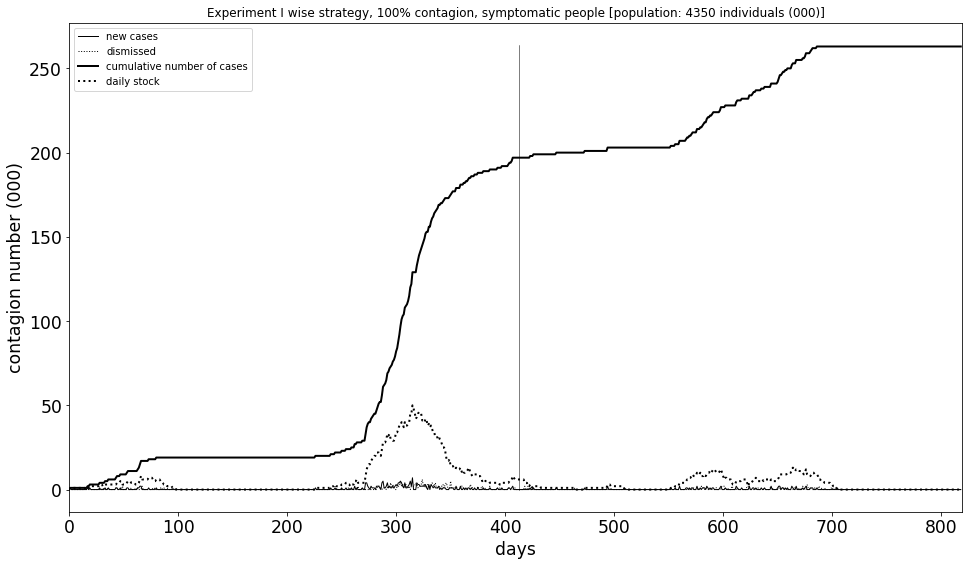
\includegraphics[scale=0.16]{Experiment_I_1_wise_symptomatic_series.png} 

\caption{``Wise'' vaccination symptomatic series; the vertical line is at day 413, when the effectiveness of first vaccination starts} 
\label{Experiment_I_wiseSymptomaticSeries}
\end{figure}



\end{frame}

%%%%%%%%%%%%%%%%%%%%%%%%%%%%%%%%%%%%%%%%%%%%%%%%%%%%%%%%%
\begin{frame}{Time dynamics with best GAs strategy, vac, people still spreading the infection}

\begin{figure}[H]
\center
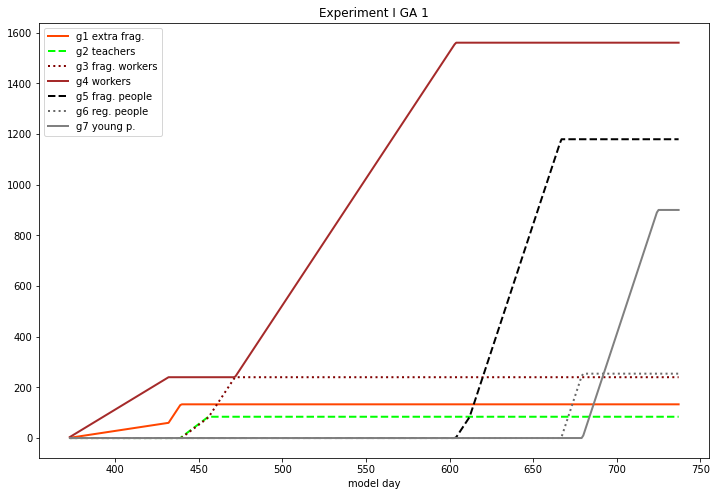
\includegraphics[scale=0.16]{Experiment_I_GA_1_VaccinationSequence.png} % experiment_I_vaccination_plots.ipynb

\caption{GA 1 vaccination sequence; on the $y$ axis the number of vaccinated subjects of each group (if vaccination is complete, the line is horizontal)} 
\label{Experiment_I_GA1VaccinationSequence}
\end{figure}

% using contagionSeriesByGroups.ipynb on Experiment_I_1bestGA.csv 
\begin{figure}[H]
\center
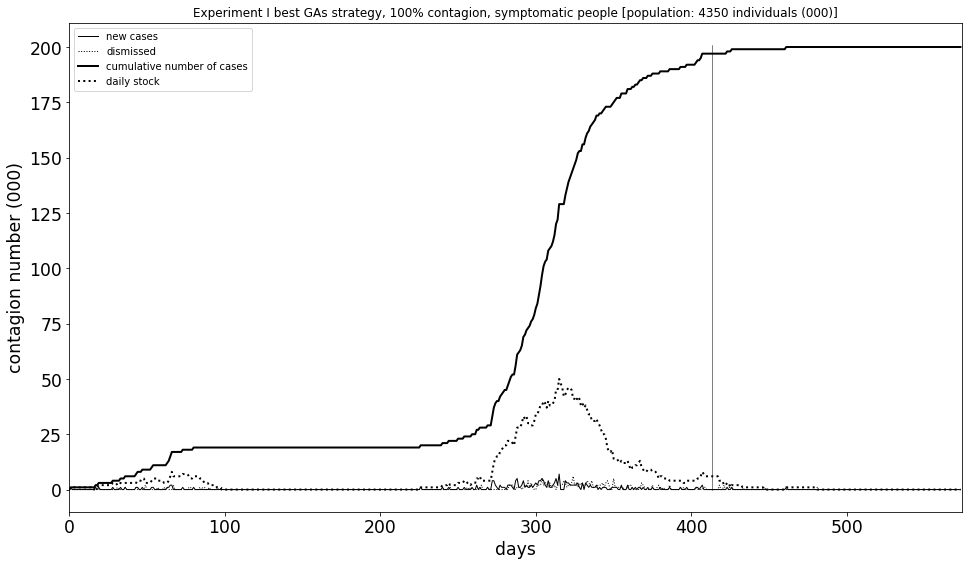
\includegraphics[scale=0.16]{Experiment_I_1_GAs_symptomatic_series.png} 

\caption{GAs vaccination symptomatic series; the vertical line is at day 413, when the effectiveness of first vaccination starts} 
\label{Experiment_I_GAs1SymptomaticSeries}
\end{figure}


\end{frame}

%%%%%%%%%%%%%%%%%%%%%%%%%%%%%%%%%%%%%%%%%%%%%%%%%%%%%%%%%
\subsection{What if}

%%%%%%%%%%%%%%%%%%%%%%%%%%%%%%%%%%%%%%%%%%%%%%%%%%%%%%%%%
\begin{frame}{What if}
\center
What if we increase quantities in \emph{plain} and \emph{wise} strategies?

\begin{table}[H]
\centering
\begin{small} % or footnotesize, scriptsize, tiny, etc.
\begin{tabular}{ccc}
\toprule
From day & Q. & Q. + \\
\midrule
373      & 5           & 10            \\
433      & 10         & 15            \\
493      & 10         & 25            \\
553      & 10         & 25            \\
613      & 20         & 25            \\
738      & end     \\ 
\bottomrule  
\end{tabular}
\end{small}
\caption{New daily quantities}
\label{quotaTablePlus}
\end{table}


\end{frame}

%%%%%%%%%%%%%%%%%%%%%%%%%%%%%%%%%%%%%%%%%%%%%%%%%%%%%%%%%

\begin{frame}{Time dynamics with \emph{plain+} vac. strategy, v. people still spreading the infection}

\begin{figure}[H]
\center
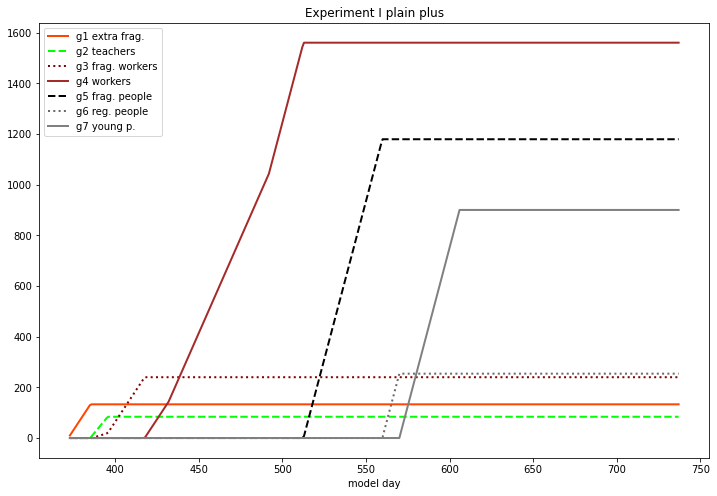
\includegraphics[scale=0.16]{Experiment_I_plainPlusVaccinationSequence.png} % experiment_I_vaccination_plots.ipynb

\caption{``Plain+'' vaccination sequence; on the $y$ axis the number of vaccinated subjects of each group (if vaccination is complete, the line is horizontal)} 
\label{Experiment_I_plainVaccinationSequence}
\end{figure}

% using contagionSeriesByGroups.ipynb on Experiment_I_plainPlus_1.csv 
\begin{figure}[H]
\center
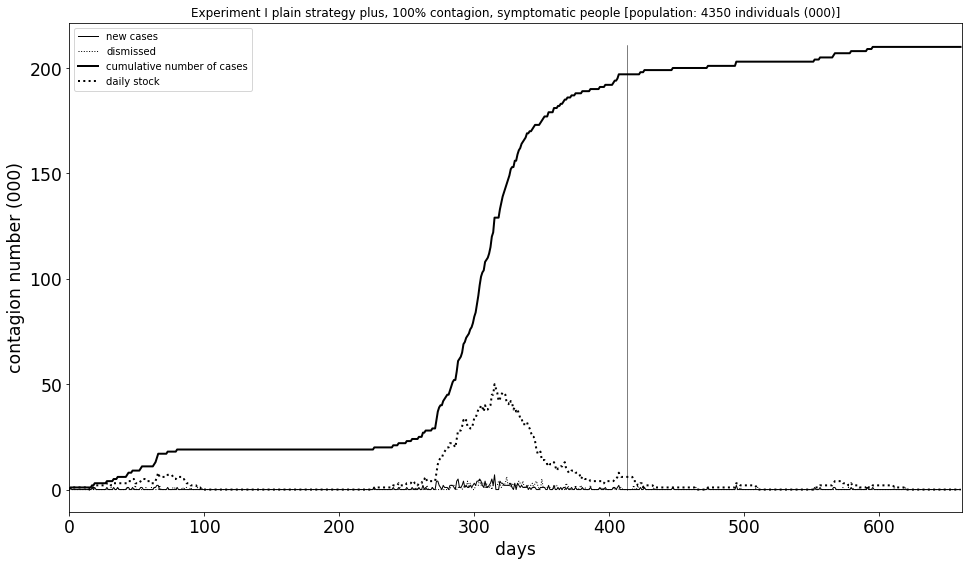
\includegraphics[scale=0.16]{Experiment_I_1_plainPlus_symptomatic_series.png} 

\caption{``Plain'' vaccination symptomatic series; the vertical line is at day 413, when the effectiveness of first vaccination starts} 
\label{Experiment_I_plainSymptomaticSeries}
\end{figure}



\end{frame}

%%%%%%%%%%%%%%%%%%%%%%%%%%%%%%%%%%%%%%%%%%%%%%%%%%%%%%%%%
\begin{frame}{Time dynamics with \emph{wise+} vac. strategy, v. people still spreading the infection}

\begin{figure}[H]
\center
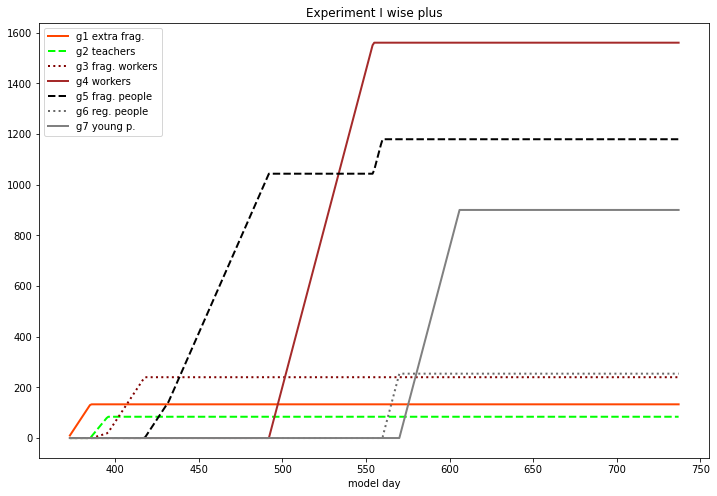
\includegraphics[scale=0.16]{Experiment_I_wisePlusVaccinationSequence.png} % experiment_I_vaccination_plots.ipynb

\caption{``Wise+'' vaccination sequence; on the $y$ axis the number of vaccinated subjects of each group (if vaccination is complete, the line is horizontal)} 
\label{Experiment_I_wiseVaccinationSequence}
\end{figure}

% using contagionSeriesByGroups.ipynb on Experiment_I_wisePlus_1.csv 
\begin{figure}[H]
\center
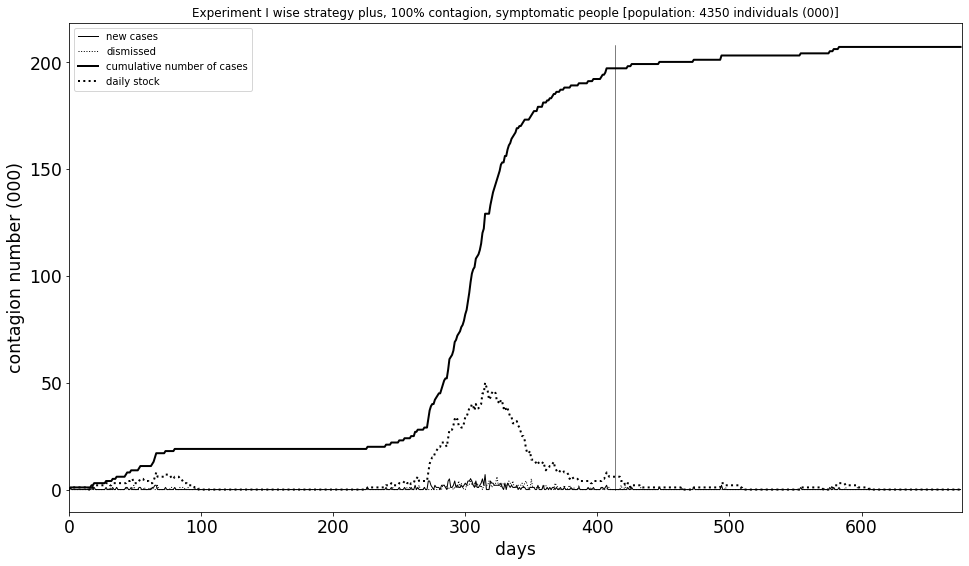
\includegraphics[scale=0.16]{Experiment_I_1_wisePlus_symptomatic_series.png} 

\caption{``Wise+'' vaccination symptomatic series; the vertical line is at day 413, when the effectiveness of first vaccination starts} 
\label{Experiment_I_wiseSymptomaticSeries}
\end{figure}



\end{frame}



%%%%%%%%%%%%%%%%%%%%%%%%%%%%%%%%%%%%%%%%%%%%%%%%%%%%%%%%%
\begin{frame}{Synopsis}

\center
Hypothesis: vaccinated people, if infected, are diffusing the contagion.

\medskip

\begin{table}[H]
\centering
%\begin{scriptsize} % or footnotesize, scriptsize, tiny, etc.
\begin{tabular}{llllllll}
\toprule
Case    & At   & Final      & Final        & Final       & Final   & Final       & Final       \\
             & day & no         & plain       & wise        & GAs       & plain  +     & wise +  \\
             & 413 & vaccin. & vaccin.    & vaccin.  & vaccin.   & vaccin.   & vaccin.      \\
 (1000) \\
\midrule
I            & 197 & 325 & 236 & 263 & \textbf{200} & 210 & 207  \\
             & -      & 128 & 39    & 66  & \textbf{3}    & 13    &  10  \\

\bottomrule  
\end{tabular}
%\end{scriptsize}
\caption{Results of the vaccination campaigns: only symptomatic people (second row: minus day 413)}
\label{caseSynopsys}
\end{table}

\end{frame}
%%%%%%%%%%%%%%%%%%%%%%%%%%%%%%%%%%%%%%%%%%%%%%%%%%%%%%%%%
\section{A new model}

%%%%%%%%%%%%%%%%%%%%%%%%%%%%%%%%%%%%%%%%%%%%%%%%%%%%%%%%%
\begin{frame}{A new model: the map}

\begin{figure}[H]
\center
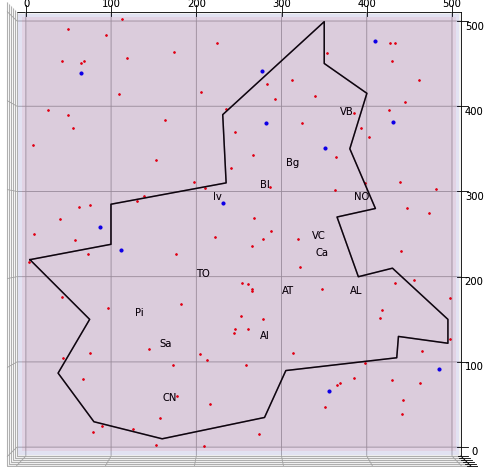
\includegraphics[scale=0.25]{Piem1.png}~~~~~~~~~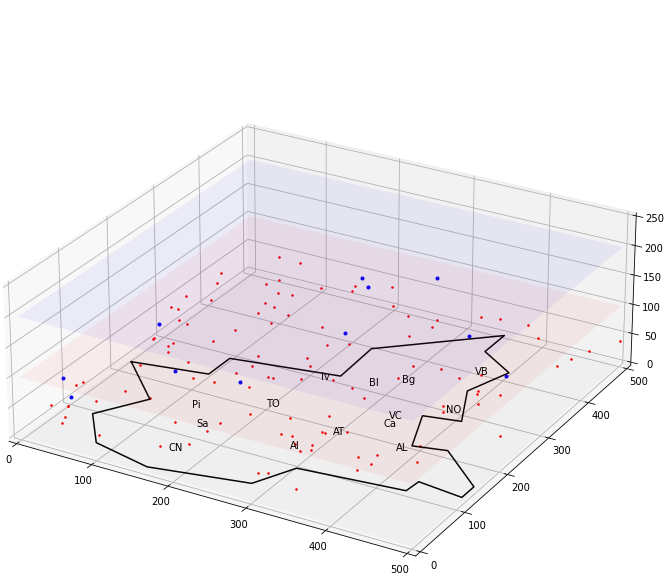
\includegraphics[scale=0.25]{Piem2.png} 

\caption{3D Piedmont} 
\label{Piem}
\end{figure}

\end{frame}

%%%%%%%%%%%%%%%%%%%%%%%%%%%%%%%%%%%%%%%%%%%%%%%%%%%%%%%%%
\begin{frame}{A new model: the scale and the items}

\begin{itemize}

\item $1:100$.

\item \textit{Infection engine}, \url{https://terna.to.it/simul/InfectionEngine.pdf}.

\item Houses.
\item Schools.
\item Hospitals.
\item Nursing homes,
\item Factories.
\color{red}
\item Transportations.
\item Aggregation places: happy hours, night life, sport stadiums, discotheques, \ldots
\color{blue}
\item Networks (family networks, professional networks, high-contact individuals,\footnote{G. Manzo and A. van de Rijt. Halting sars-cov-2 by targeting high-contact individuals. Journal of Artificial Societies and Social Simulation, 23(4):10, 2020. ISSN 1460-7425. doi: 10.18564/jasss.4435. URL http://jasss.soc.surrey.ac.uk/23/4/10.html.} \ldots) 

\end{itemize}

\end{frame}

%%%%%%%%%%%%%%%%%%%%%%%%%%%%%%%%%%%%%%%%%%%%%%%%%%%%%%%%%
\begin{frame}{The tool: S.L.A.P.P.}

Scientific advertising: \url{https://terna.github.io/SLAPP/}

\begin{figure}[H]
\center

\includegraphics[scale=0.26]{SLAPP.png}

\caption{Swarm-Like Agent Protocol in Python} 
\label{SLAPP}
\end{figure}

\end{frame}

%%%%%%%%%%%%%%%%%%%%%%%%%%%%%%%%%%%%%%%%%%%%%%%%%%%%%%%%%
\section{Agricultural field}

%%%%%%%%%%%%%%%%%%%%%%%%%%%%%%%%%%%%%%%%%%%%%%%%%%%%%%%%%
\begin{frame}{ABMs in agricultural field}

An offer of cooperation.

% https://scholar.google.it/scholar?hl=it&as_sdt=0%2C5&q=agent-based+model+Precision+agriculture&btnG=

\end{frame}

%%%%%%%%%%%%%%%%%%%%%%%%%%%%%%%%%%%%%%%%%%%%%%%%%%%%%%%%%
\begin{frame}{Examples in agricultural field (1/5)}

\begin{figure}[H]
\center
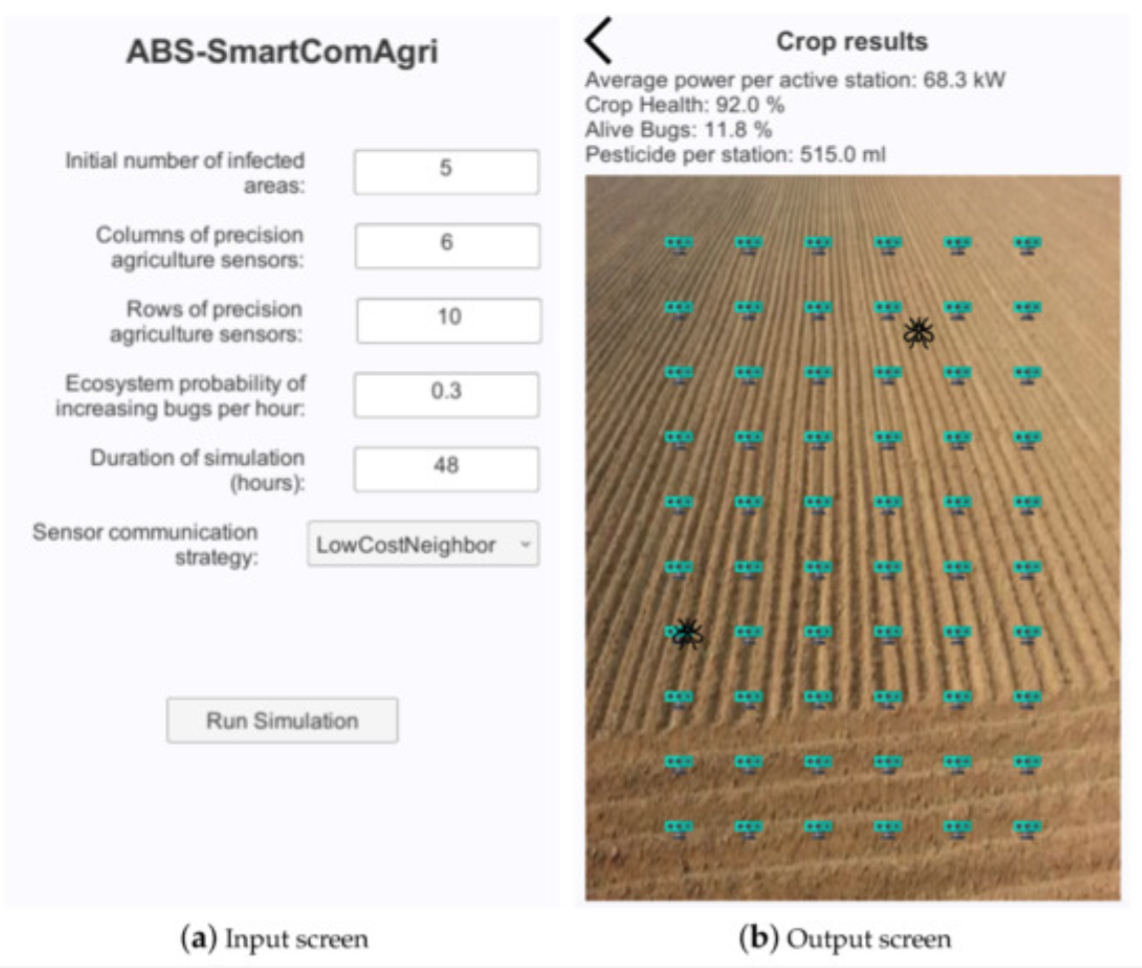
\includegraphics[scale=0.32]{agr1.png}
\label{agr1}
\end{figure}

\href{https://www.mdpi.com/1424-8220/18/4/998}{ABS-SmartComAgri: An Agent-Based Simulator of Smart Communication Protocols in Wireless Sensor Networks for Debugging in Precision Agriculture}

\end{frame}

%%%%%%%%%%%%%%%%%%%%%%%%%%%%%%%%%%%%%%%%%%%%%%%%%%%%%%%%%
\begin{frame}{Examples in agricultural field (2/5)}

\begin{figure}[H]
\center
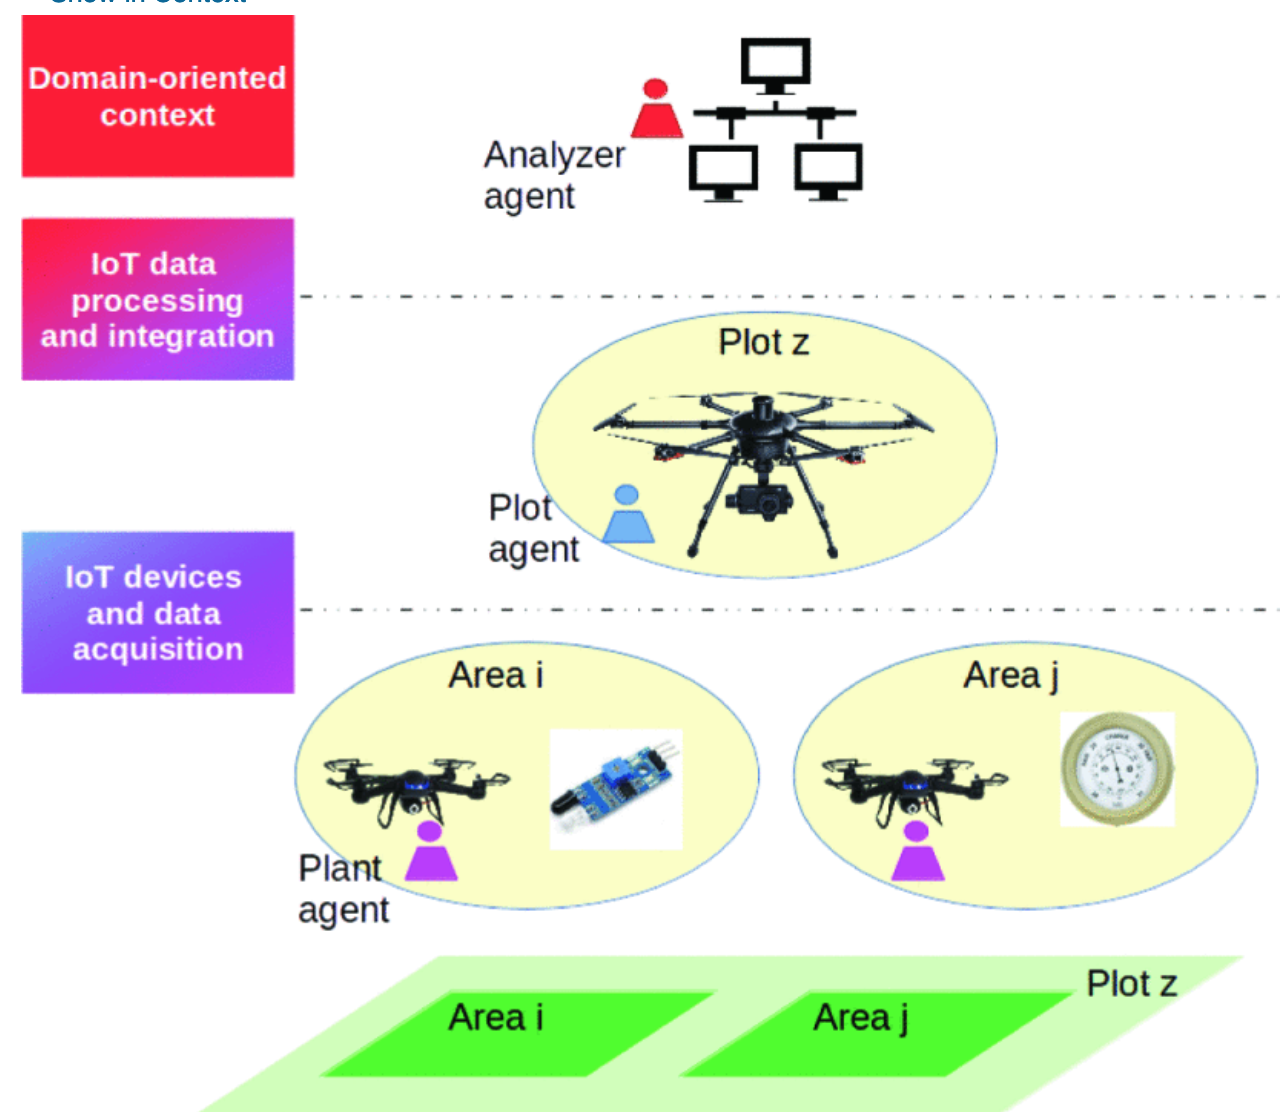
\includegraphics[scale=0.32]{agr2.png}
\label{agr2}
\end{figure}

\href{https://ieeexplore.ieee.org/abstract/document/9177771}{Towards a layered agent-modeling of IoT devices to precision agriculture}

\end{frame}

%%%%%%%%%%%%%%%%%%%%%%%%%%%%%%%%%%%%%%%%%%%%%%%%%%%%%%%%%
\begin{frame}{Examples in agricultural field (3/5)}

\begin{figure}[H]
\center
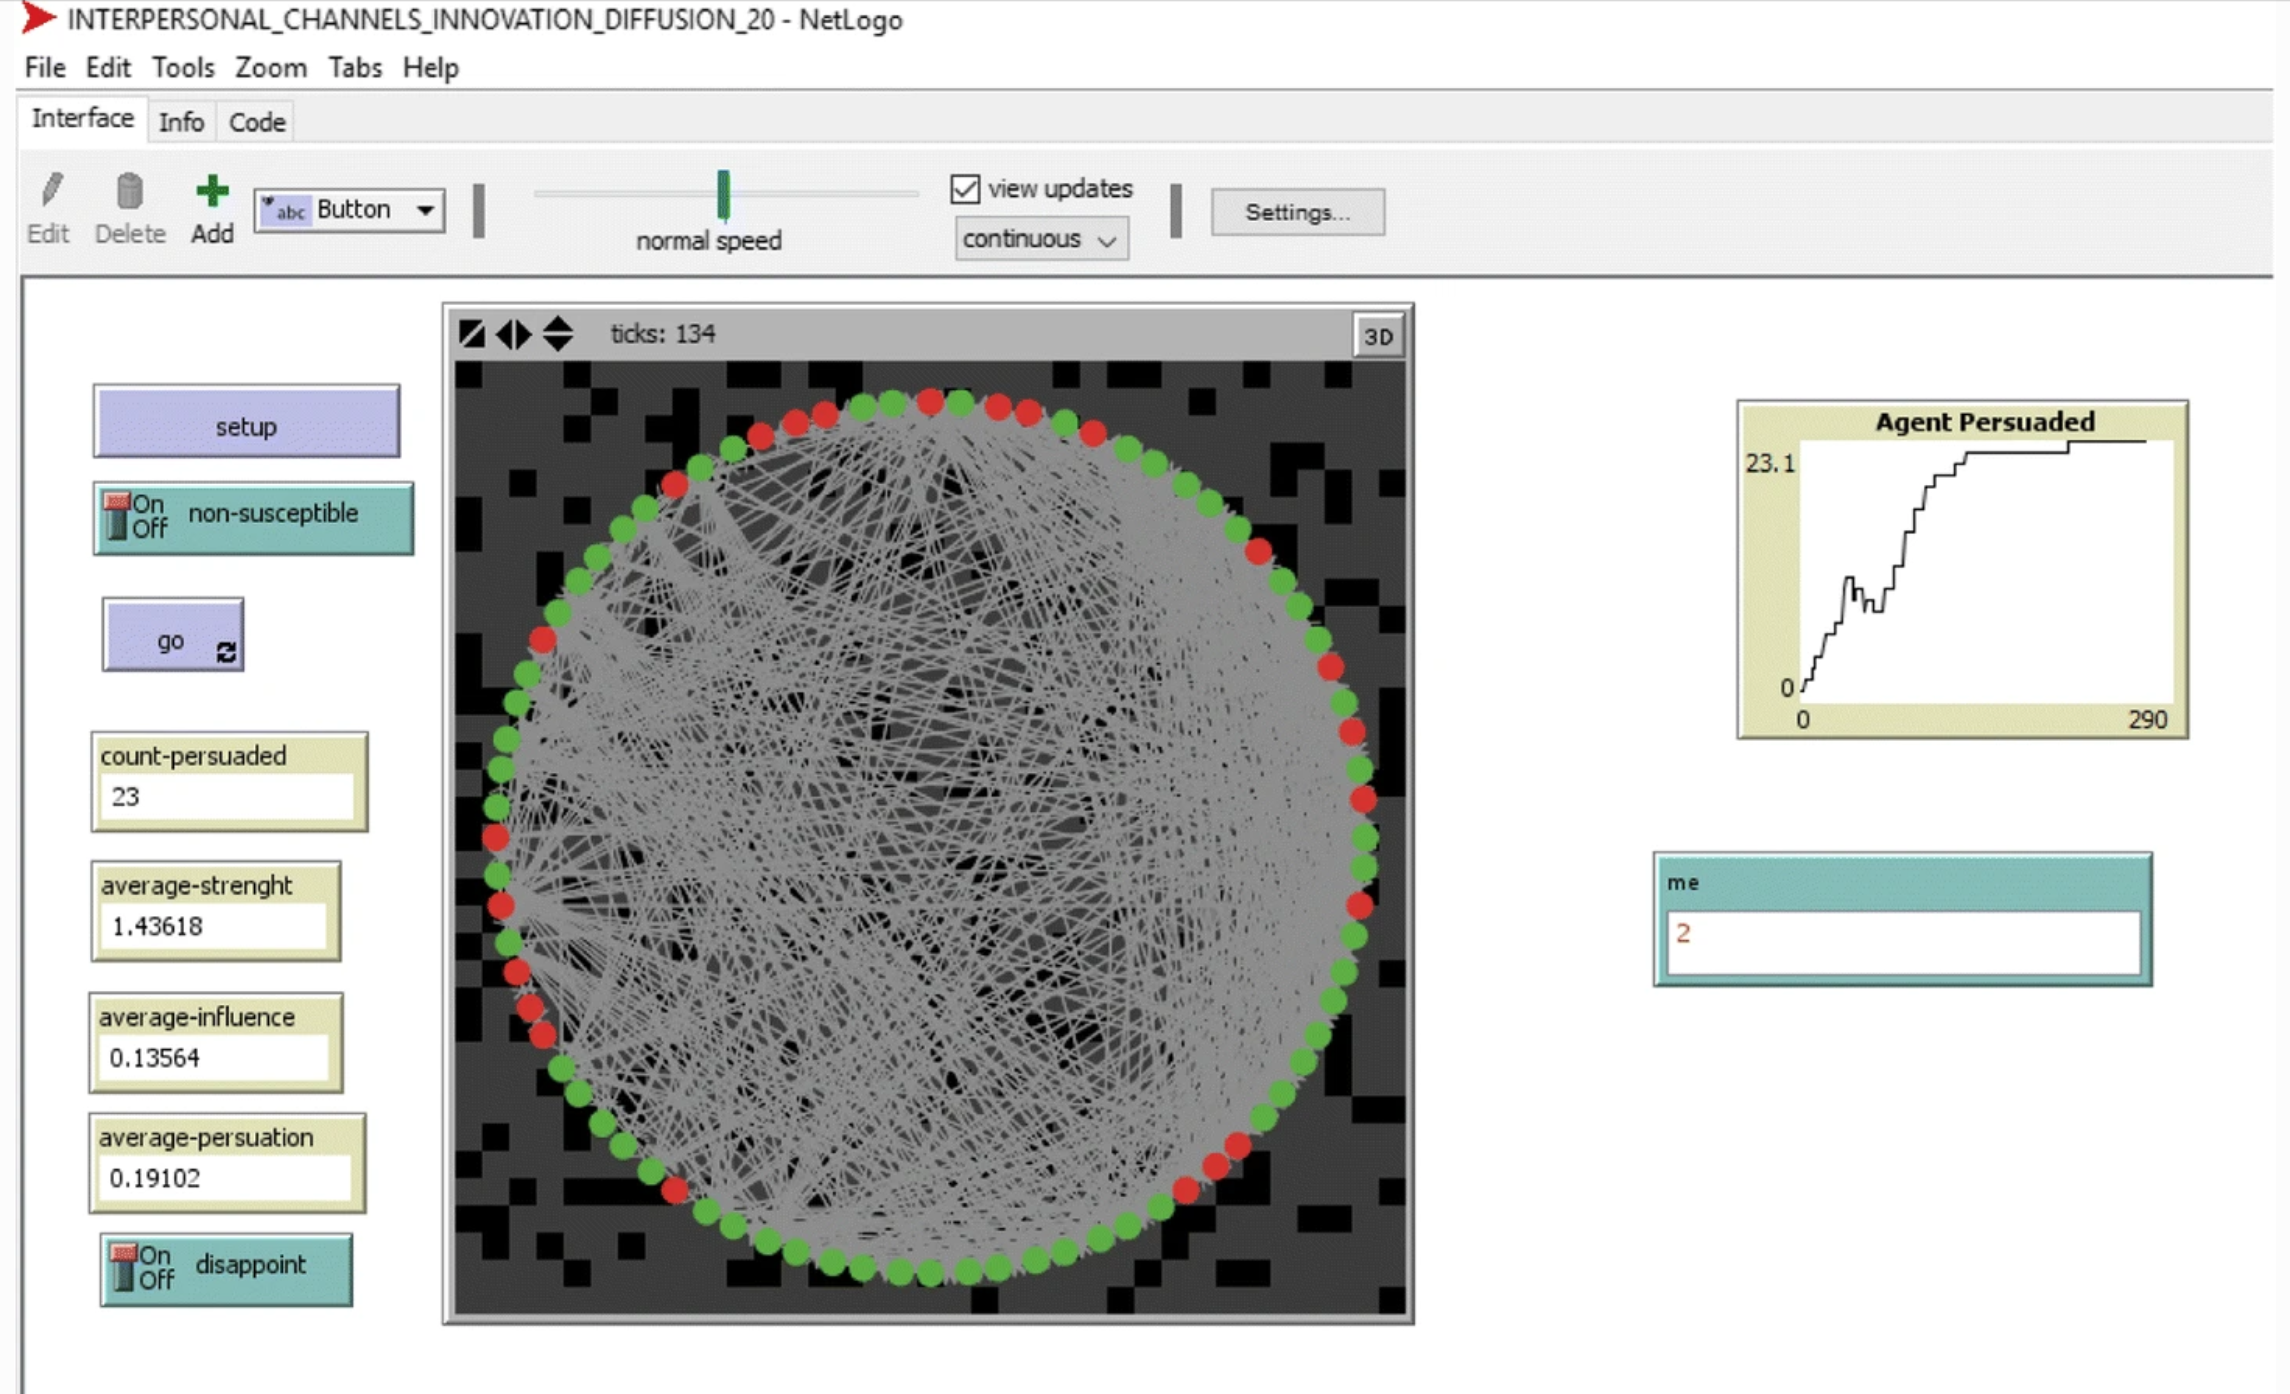
\includegraphics[scale=0.25]{agr3.png}
\label{agr3}
\end{figure}

\href{https://link.springer.com/article/10.1186/s40100-019-0121-0}{Improving diffusion in agriculture: an agent-based model to find the predictors for efficient early adopters}

\end{frame}

%%%%%%%%%%%%%%%%%%%%%%%%%%%%%%%%%%%%%%%%%%%%%%%%%%%%%%%%%
\begin{frame}{Examples in agricultural field (4/5)}

\begin{figure}[H]
\center
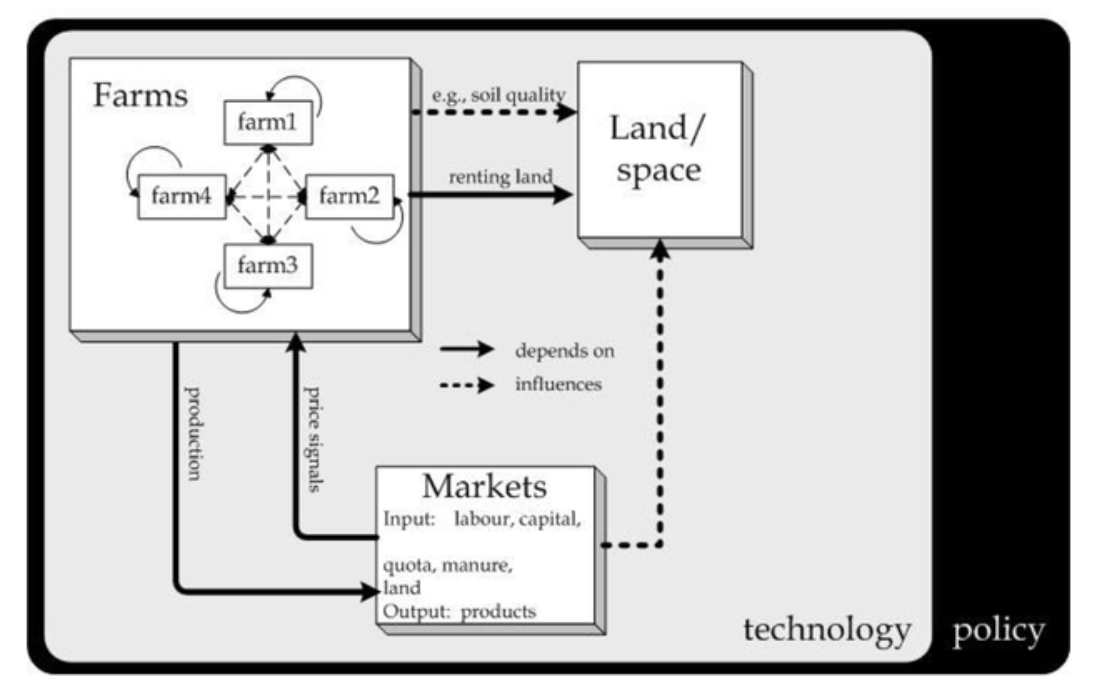
\includegraphics[scale=0.36]{agr4.png}
\label{agr4}
\end{figure}

\href{https://www.jstor.org/stable/26267800}{Agent-based Analysis of Agricultural Policies: an Illustration of the Agricultural Policy Simulator AgriPoliS, its Adaptation and Behavior}

\end{frame}

%%%%%%%%%%%%%%%%%%%%%%%%%%%%%%%%%%%%%%%%%%%%%%%%%%%%%%%%%
\begin{frame}{Examples in agricultural field (5/5)}

\begin{figure}[H]
\center
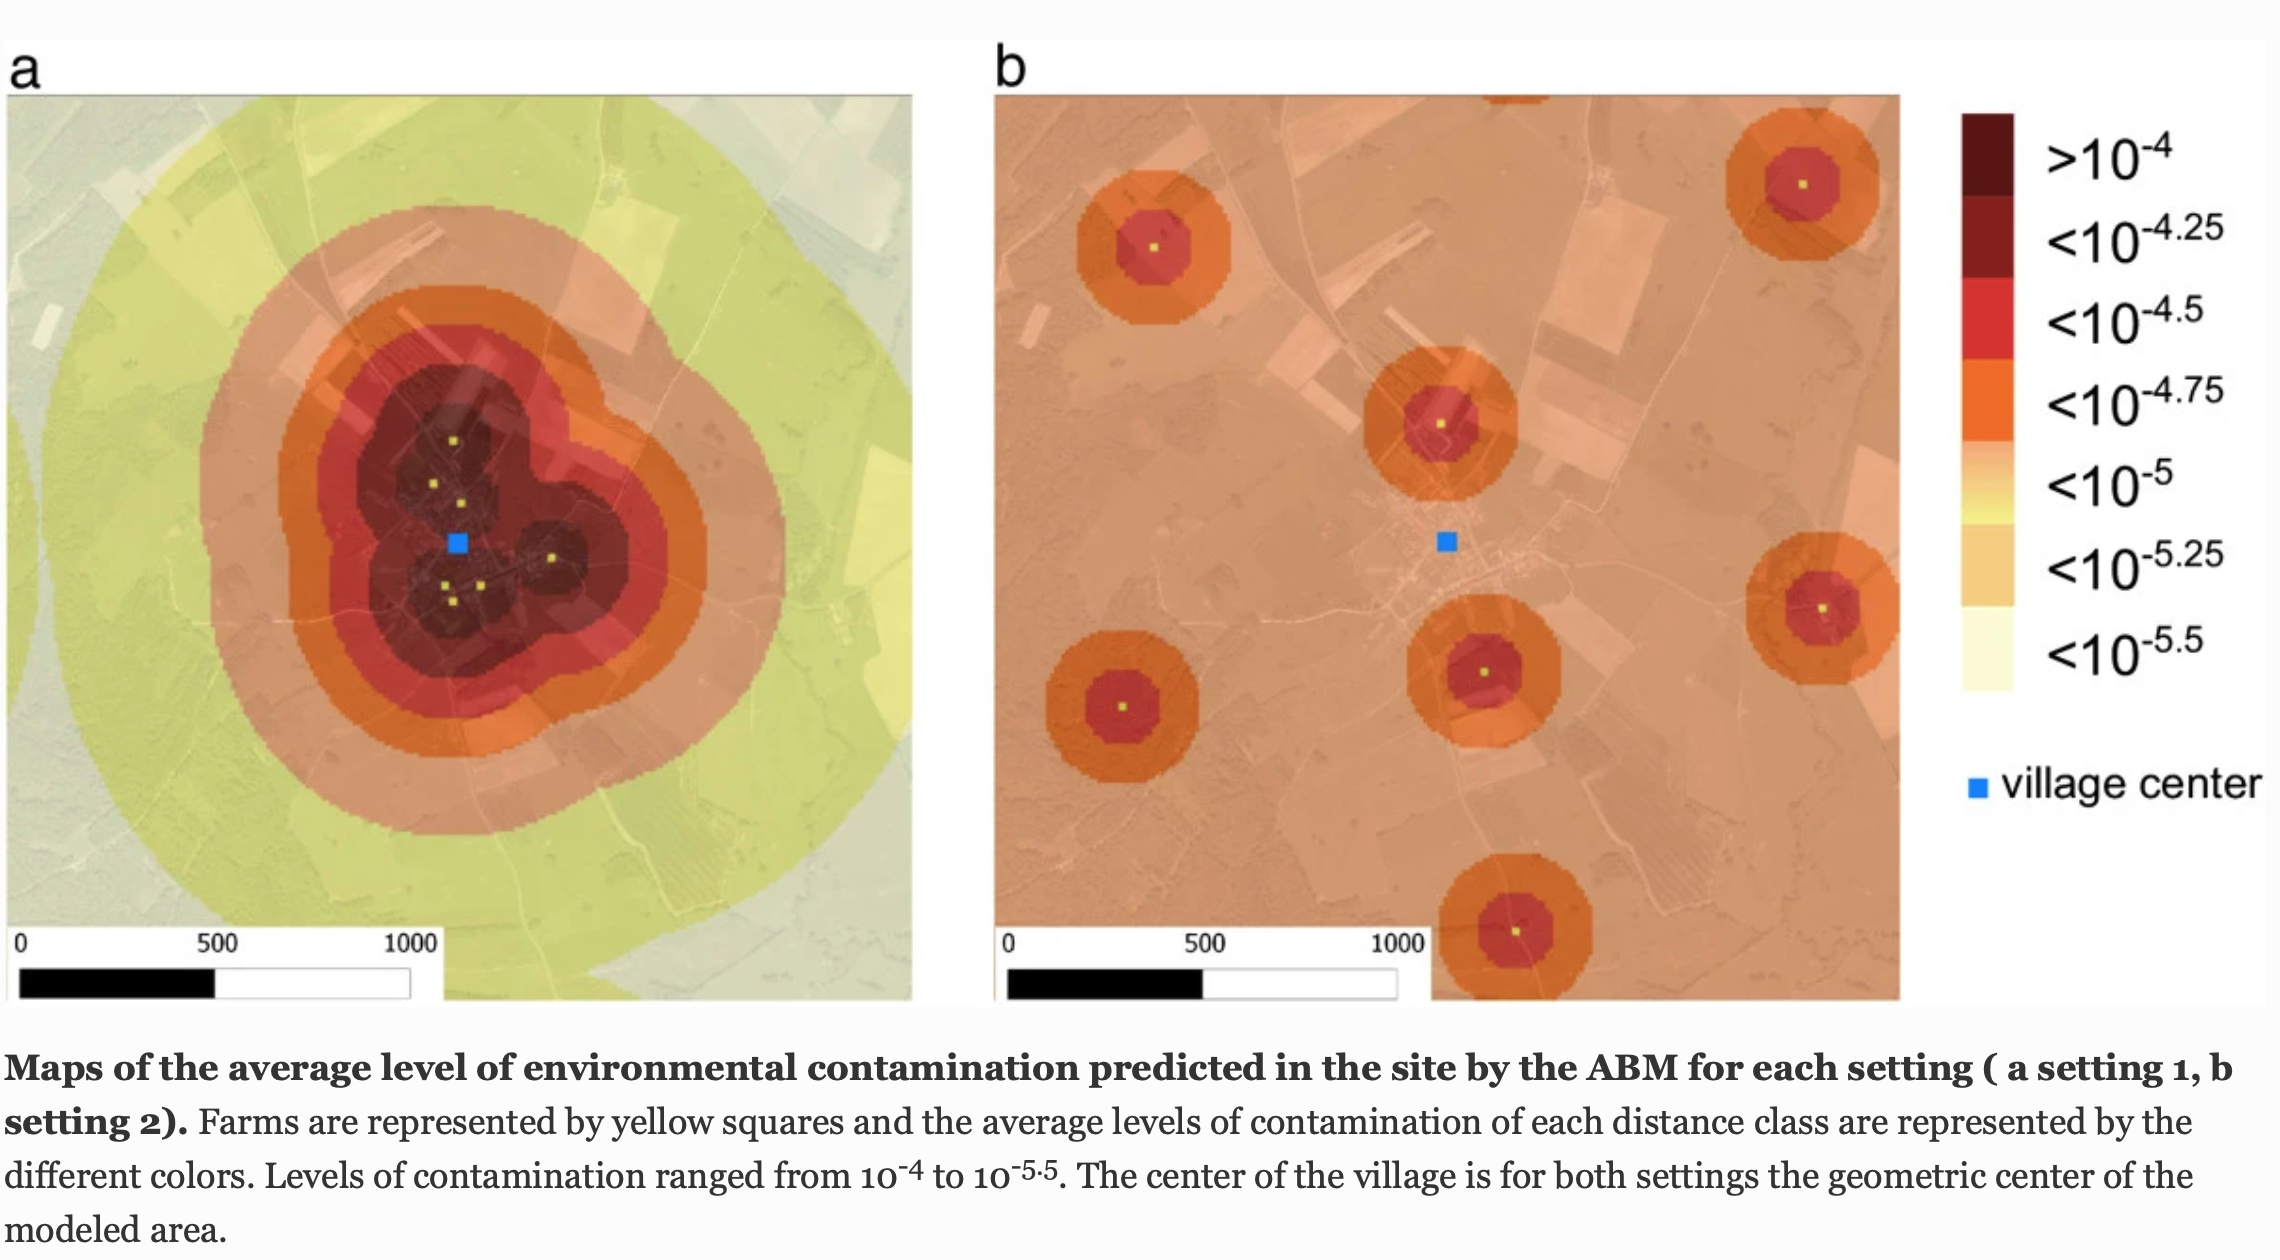
\includegraphics[scale=0.25]{agr5.png}
\label{agr5}
\end{figure}

\href{https://link.springer.com/article/10.1186/1476-072X-13-45}{Agricultural landscape and spatial distribution of \emph{Toxoplasma gondii} in rural environment: an agent-based model}

\end{frame}

%%%%%%%%%%%%%%%%%%%%%%%%%%%%%%%%%%%%%%%%%%%%%%%%%%%%%%%%%
\begin{frame}{}


Many thanks.

\bigskip

Slides at \url{https://terna.to.it/aa.pdf}.

\bigskip

Home page at \url{https://terna.to.it}.


\end{frame}


\end{document}